
\documentclass[10pt]{amsart}
\usepackage[left=.5in,right=.5in,top=.5in,bottom=.5in]{geometry}
\geometry{letterpaper}                   % ... or a4paper or a5paper or ... 
%\geometry{landscape}                % Activate for for rotated page geometry
%\usepackage[parfill]{parskip}    % Activate to begin paragraphs with an empty line rather than an indent
\usepackage{color,graphicx}
\usepackage{amssymb}
\usepackage{amsmath}
\usepackage{epstopdf}
\usepackage[]{algorithm2e}
\DeclareGraphicsRule{.tif}{png}{.png}{`convert #1 `dirname #1`/`basename #1 .tif`.png}
\newcommand{\eqn}[1]{(\ref{#1})}
\newcommand{\picdir}{./pdffig}
\renewcommand{\labelenumi}{\arabic{enumi}. }

\title{Accelerated and Validated Model Based MR Signal Recon}

\begin{document}
\maketitle

%%%%%%%%%%%%%%%%%%%%%%%%%%%%%%%%%%%%%%%%%%%%%%%%%%%%%%%%%%%%%%%%%%%%%%%%%%%%%%%%
\section{Background Reading}
%%%%%%%%%%%%%%%%%%%%%%%%%%%%%%%%%%%%%%%%%%%%%%%%%%%%%%%%%%%%%%%%%%%%%%%%%%%%%%%%
  \begin{itemize}
    \item MR signal model derivation~\cite{Haacke1999,Bernstein2004}.
          Equations for model based processing of the MR Signal is provided in Section~\ref{ModelBasedProcessing}.
    \item Signal equation from a digital signal processing perspective~\cite{candy2005model}. 
    \item Statistical Inverse Problem Framework \cite{tarantola05}.  
          Laplacian distribution~\cite{Eltoft2006,Babacan2010}.
    \item CS Background~\cite{Fessler2010b,Donoho2006a,Candes2008}.
  \begin{itemize}
    \item  Suppose we are given a signal $x \in \mathbb{R}^m$ and a basis
           $\theta_i = <\varphi_i,x> $ $i = 1,...,N$ in which the signal is
           sparse, ie that  the 1-norm is bounded
           \[
              \|\theta\|_1 \leq R
           \]
           Given $n = N \; log \;m $ measurements, $\theta_1, .... \theta_n$, the approximation
           of the solution $\bar{x}$ computed as the solution to the L1
           problem is of the same quality (with respect to the 2-norm) as 
           using the $N$ largest coefficients. ie 
           \[
             \| x - \bar{x}\| \leq C  \frac{1}{\sqrt{N}}
           \]
           ie there is little benefit, in terms of solution accuracy, if we
           were to wait longer to collect all measurement coefficients.
           This is similar to an iterative solver where a handful of matrix
vector product product a solution accuracy $\mathcal{O}(10^{-6})$ precision with $\mathcal{O}(N)$ 
complexity and there is really no need to use a direct solver
to get a $\mathcal{O}(10^{-16})$ precision with $\mathcal{O}(N^3)$
complexity. 
     \item As a big surprise, From \cite{Donoho2006a}, "So adaptive information is of minimal help—despite the quite
natural expectation that an adaptive method ought to be able
iteratively somehow "localize" and then "close in" on the "big
coefficients."
   \[
     \text{error non-adaptive} \leq Const. \; \cdot \; \text{error adaptive}
   \]
  \end{itemize}
    \item Model Based CS~\cite{Baraniuk2010}.
  \begin{itemize}
    \item In order to get a good approximation, the measurement matrix 
         $\Phi = \left[\varphi_1 .. \varphi_N \right]$ should satisfy the restricted
          isometry property (RIP)
          \begin{equation} \label{RIPMatrix}
           (1-\delta_k) \|x\|_2 \leq \|\Phi x\| \leq (1+\delta_k) \|x\|_2
          \end{equation}
          The RIP property ensures that submatrices are close to an isometry
          and are thus information preserving.
  \end{itemize}
    \item Model based CS Recon Applications in MR~\cite{Cao2014,Wright2014,Asslander2013}.
    \item GPU Code~\cite{Farber2011a,Munshi2011,Hansen2013}.
    \item Computational Harmonic Analysis is an active field of research to
determine basis functions with rapidly decaying
coefficients~\cite{feichtinger1989atomic,candes2004new}.
    \item Dictionaries provide an alternative view for construction a basis
          for the sparse reconstruction~\cite{Candes2011,Aharon2006,Elad2006}.
         \begin{itemize}
             \item From \cite{Elad2006} "with the growing realization that regular
separable 1-D wavelets are inappropriate for handling images, several new tailored multiscale and directional redundant
transforms have been introduced, including the curvelet \cite{candes2002recovering,candes2004new},
contourlet \cite{do2003contourlets,do2003framing}, wedgelet \cite{donoho1999wedgelets}, 
bandlet\cite{le2005sparse,le2005bandelet} , and the steerable wavelet \cite{freeman1991design,simoncelli1992shiftable}."
         \end{itemize}
    \item Markov Chain Monte Carlo (MCMC) was placed in the top 10 most important algorithms of the
	  20th century~\footnote{http://www.siam.org/pdf/news/637.pdf}.  The
          basic idea behind MCMC is to construct a Markov chain  on the state space
          whose stationary distribution is the target density of
          interest, Ch 24 \cite{Murphy2012a}.
  \end{itemize}


%%%%%%%%%%%%%%%%%%%%%%%%%%%%%%%%%%%%%%%%%%%%%%%%%%%%%%%%%%%%%%%%
\section{Mathematical Framework}\label{GeneralMathFramework}
%%%%%%%%%%%%%%%%%%%%%%%%%%%%%%%%%%%%%%%%%%%%%%%%%%%%%%%%%%%%%%%%

The underlying modeling philosophy of the presentation is that the physics 
models are 1st order accurate or within 70-80\% of the needed accuracy and the error "is
within" Gaussian noise.
Gaussian distributions provide analytical representations of the random
variables of interest within the Bayesian setting and 
provide a crux for understanding. In particular, we say that a random
variable $\eta$ belongs to a multi-variate normal distribution 
of mean $\mu \in \mathbb{R}^n $ and covariance $\Sigma \in \mathbb{R}^{n \times n}$
\[
     \eta \sim \mathcal{N}(\mu,\Sigma)  
    \Rightarrow
      p(\eta)  = \frac{1}{2 \; \pi \; \det{\Sigma}} \exp\left( - \frac{1}{2} \| \mu - \eta\|^2_{\Sigma}\right)
\]


\begin{enumerate}
  \item We will consider multiple physics/sensor models,
$\mathcal{G}_i(\vec{k},\theta): \mathbb{R}^a
\times \mathbb{R}^m \rightarrow \mathbb{R}^n $, $i=1,..., N_\text{model}$.
Each model $\mathcal{G}_i$ maps deterministic acquisition
parameters, $\vec{k} \in \mathbb{R}^a$, and uncertain parameters, $\theta \in \mathbb{R}^m$
to observables, $\vec{z} \in \mathbb{R}^n$ ( or $\vec{z} \in \mathbb{C}^n$).
To be explicit, will assume that the
measurement models are corrupted by zero mean white noise noise of a
\textbf{known} covariance matrix, $\Sigma_z \in \mathbb{R}^{n \times n}$ 
\begin{equation}
\label{sensormodelstructure}
    \vec{z} = \mathcal{G}_i(\vec{k};\theta) + \eta   \qquad   \eta \sim \mathcal{N}(0,\Sigma_z) 
\end{equation}
$\eta$ may be interpreted as the measurement noise or the acquisition noise
in the sensor model. For a deterministic measurement model $\mathcal{G}$,
the conditional probablity distribution has an explicit analytical form
and may be written as a  \textbf{known} Gaussian
distribution. 
  \[
      p(\vec{z}|\theta) =  \mathcal{N}(\mathcal{G}_i(\vec{k};\theta),\Sigma_z)  \qquad 
                                                           i=1,..., N_\text{model}
  \]
This model corresponds to the fifth sketch in
Figure~\ref{InverseProblemSummary} (\cite{tarantola05} Figure 3.2). 
Generally, this is a nonlinear model in 
which linear approximations are not appropriate.
\begin{figure}[h]
\centering
\scalebox{0.52}{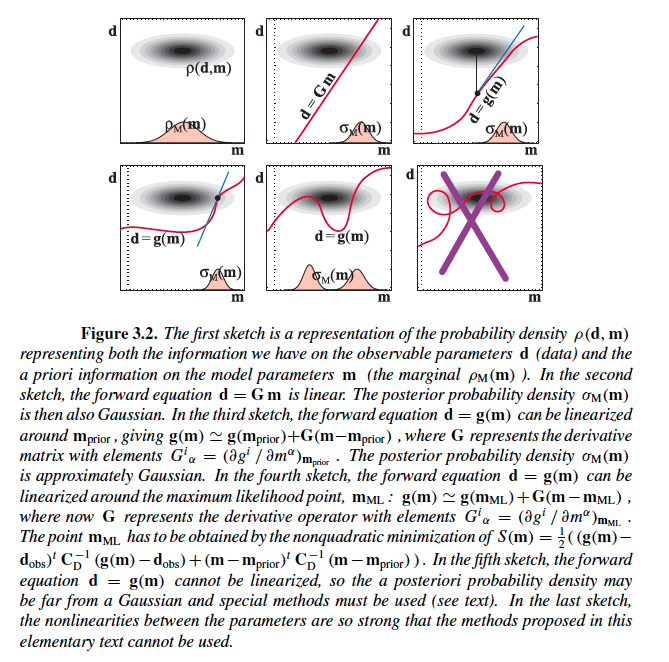
\includegraphics{\picdir/InverseProblemSummary}}
\caption{\cite{tarantola05} Figure 3.2.
     Different models include: single echo, multi-echo, multi-flip,
motion correction, and sparsity. The models may be linear or nonlinear.
} \label{InverseProblemSummary}
\end{figure}
  \item Additional \textbf{known} information is the prior probability
distributions for the model parameters, $p(\theta)$. 
   \begin{itemize}
    \item Prior parameters may be a Gaussian distribution of 
   \textbf{known} mean, $\hat{\theta}$ and covariance, $\Sigma_\theta$
   \[
      \theta \sim \mathcal{N} (\hat{\theta}, \Sigma_\theta)
   \]
    \item Sparsity in the model parameters may also be an appropriate assumption.
Assume model parameters, $\theta$ are sparse under a given transformation
$\Phi$.
A Laplacian distribution 
of \textbf{known} mean, $\hat{w}$ and covariance, $\Sigma_w$
is defined in terms of $\|\cdot\|_1$ and is known to enforce
sparsity~\cite{Aravkin2011,Aravkin2011a}.
\[
   w = \Phi \theta
    \qquad
     w \sim \mathcal{L}(\hat{w},\Sigma_w)  
    \Rightarrow
      p(w)  = \frac{1}{ \sqrt{\det\left(2 \; \Sigma_w\right)}} 
                   \exp\left( -\sqrt{2} 
          \left\| 
        \Sigma_w^{-1/2} \left(w - \hat{w}\right)
         \right\|_1
                   \right)
\]
Within a compressed sensing setting, we typically  assume
the each component of the representation is \textbf{independent}
with known covariance, $\lambda$ and zero mean $\hat{w}=0$.
\[
    p(w) = \prod_i  \frac{1}{\sqrt{2 \; \lambda} }
                   \exp\left( 
                  - \frac{\sqrt{2} |w_i|}{\lambda}
                   \right)
\]
\textit{Intuitively, for a sparse representation,
the probability that an individual independent component is zero
is very high.} However, the heavy tail promotes/allows outliers
which is representative of the non-zero components.
I.e. compared to a Gaussian the probability of an outlier is greater.
\[
   \exp(-x^2) < \exp(-|x|)  \qquad x > 1
\]
{\color{red}  @dmitchell412 - TODO - validate the Laplacian assumption
on various sparsity models. Given a transformation $\Phi_i$,
\[
   w = \Phi_i \; \theta
\]
each $w_i$ is assumed independent. Statistical moments
of the histograms of the $w_i$'s should resemble a Laplacian distribution.
Can the independent assumed be evaluated within this setting as well ? 
}
\begin{figure}[h]
\centering
\scalebox{0.72}{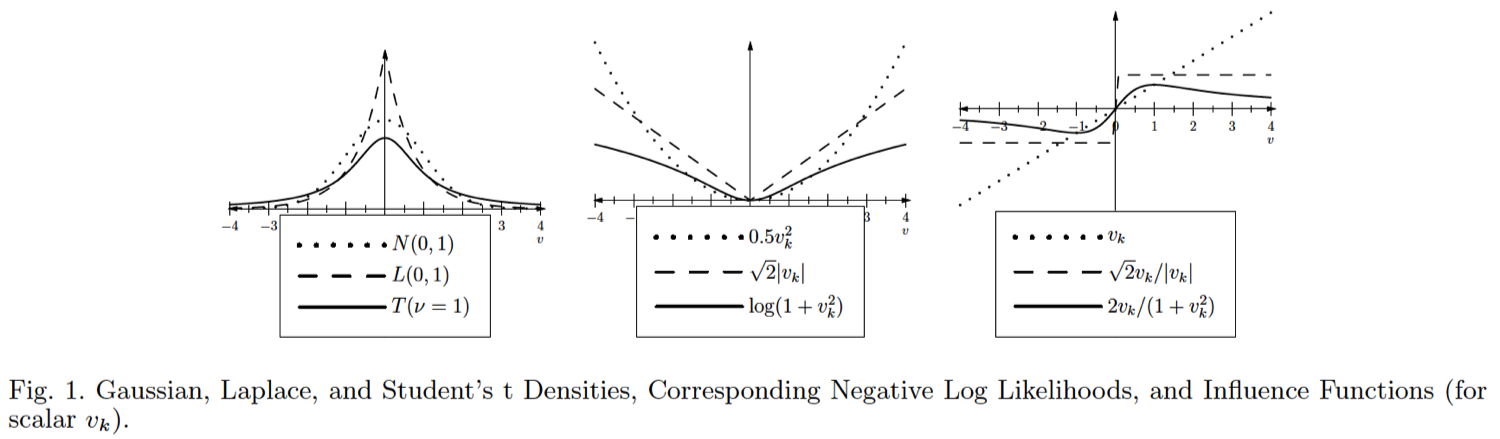
\includegraphics{\picdir/GaussLaplaceStudentDistribution}}
\caption{ \cite{Aravkin2011,Aravkin2011a}. Figure 1.  Comparison of pdf.
} \label{DistributionComparison}
\end{figure}

   \end{itemize}
  \item For each model, $\mathcal{G}_i(\vec{k};\theta)$, 
 determine the optimal measurement locations, $\vec{k}$.
This may be determined by maximizing the mutual information between
measurements, $z$, and parameters $\theta$.
The mutual information between parameters $\theta$ and $z$ may be computed as
the KL distance between the joint and independent probabilities.
\[
I(\Theta,Z) = D_\text{KL}(p(\theta,z)||p(\theta)p(z)) =  \int_z \int_\theta p(\theta,z) \ln\left(\frac{p(\theta,z)}{p(\theta)p(z)}\right) \; d\theta \; dz
\]
Motivation for this `distance'/divergence measure may be understood from information
theory~\cite{Pluim2003,Cover2006}. Given a probability space 
$(\Omega, \mathcal{F},p)$ (probability maps from the
sigma-algebra of possible events $p:\mathcal{F}\rightarrow [0,1]$
sigma-algebra, $\mathcal{F}$, defined on set of `outcomes' $\Omega$
\cite{durrett2010probability}),
we will define information of an event  as
proportional to the inverse probability.
{\color{red}  
\[
\text{information} \equiv  \frac{1}{p(\theta)}
\]
}
Intuitively, when a low probability event occurs this provides high
information.
The informational entropy is an \textit{average}
of the information content for a sigma algebra of events $\mathcal{F}$
\[
H(\Theta) = \int_\theta p(\theta) \ln\frac{1}{p(\theta)}
\]
Hence this entropy measure is an average of the information content
for a given set of events, $\mathcal{F}$, and is proportional to the
variance or uncertainty in which the set of events occur.
This agrees with thermodynamic entropy;
if the information containing events are completely spread out such as in a
uniform distribution, the entropy is maxmized.
The entropy
is zero for a probability distribution in which
only one event occurs. Zero information is gained when the same event
always occurs ($0 \ln\frac{1}{0} = 0$). 
Entropy provides an intuitive interpretation of mutual information.
\[
\begin{split}
I(\Theta,Z) 
  & = \int_z \int_\theta 
    p(\theta,z) \ln\left(\frac{p(\theta,z)}{p(\theta)p(z)}\right) \; d\theta \; dz
 = \int_z \int_\theta 
    p(\theta,z) \ln\left(\frac{p(z|\theta)}{p(z)}\right) \; d\theta \; dz
  \qquad p(\theta,z)  = p(z|\theta) p(\theta)
\\
& =  - \int_z \ln p(z)        \int_\theta 
       p(\theta,z) \; d\theta \; dz
     + \int_\theta 
       p(\theta)
       \int_z 
       p(z|\theta) \ln p(z|\theta) \; d\theta \; dz
\\
& =  - \int_z p(z) \ln p(z)       \; dz
     + \int_\theta 
       p(\theta)
       H(Z|\Theta= \theta)
    \qquad
     p(z) \equiv \int_\theta p(\theta,z) \; d\theta  
\\
& =  H(Z) - H(Z|\Theta)
\qquad
\text{
The conditional entropy, $H(Z|\Theta)$, is the average  of $ H(Z|\Theta = \theta)$.
}
\end{split}
\]
With this expression the mutual information,  $I(\Theta,Z)$,
"translates to the amount of uncertainty about the measurements $Z$
minus the uncertainty about the measurements $Z$ when the model parameters
$\Theta$ are known. In other words, MI is the amount by which the uncertainy
about the measurements $Z$ decreases when the model parameters $\Theta$ are
given: the amount of information the model parameters $\Theta$ contains
about $Z$"~\cite{Pluim2003}.
 
{\color{red}
With this interpretation in mind, we want to find acquisition parameters,
$\vec{k}$, for which the model parameters, $\Theta$, contains the most 
information about the measurements $Z$. Similarly, find acquisition parameters, $\vec{k}$, that decrease
the spread of measurement information given model prediction parameters $\Theta$.
\[
 H(Z|\Theta) = 
       \int_\theta 
       p(\theta)
       \int_z 
       p(z|\theta) \ln p(z|\theta) \; d\theta \; dz
\]
Notice that the conditional entropy is an average of an average.
The average measurment information given model parameter $\theta$ is computed for each model
parameter $\theta$. Then entropy for each $\theta$ is averaged.
The decrease in the spread of information is evaluated with respect to
the marginalized spread of measurement $Z$ information, $H(Z)$.
}

Other measures of distances to maximize joint information are the
Cauchy-Schwarz divergence~\cite{Kampa2011} 
\[
D_\text{CS}(p(\theta,z)||p(\theta)p(z)) =  -\ln\left(
\frac{\int_z \int_\theta p(\theta,z) p(\theta)p(z) \; d\theta \; dz}
     {\int_z \int_\theta p^2(\theta,z) \; d\theta \; dz \int_z \int_\theta p^2(\theta)p^2(z) \; d\theta \; dz}
\right) 
\]
and the Jensen-Renyl divergence~\cite{hamza2003jensen}
\[
D_\text{JR}(p(\theta,z)||p(\theta)p(z)) =   ? 
\]


\fbox{\begin{minipage}{.9\textwidth}
Bayes theorem is fundamental to the approach.
\[
p(y|x) p(x) = p(x,y) = p(x|y) p(y)
\]
{\color{red}  @dmitchell412 - TODO - provide an intuitive interpretation of Bayes
rule and an intuitive interpretation of conditional probability using Gaussian distributions}
\end{minipage} }

Bayes rule may be applied to simplify this expression
to the expected value of the KL-distance
\[
p(\theta,z) = p(\theta|z) \; p(z)
            = p(z|\theta) \; p(\theta)
\]
\begin{equation}
\label{mutualinformation}
\begin{split}
I(\theta,z) &= \int_z \int_\theta p(z|\theta) p(\theta) \ln\left(\frac{p(z|\theta)p(\theta)}{p(\theta)p(z)}\right)  \; dz\; d\theta
\\
            &= \int_\theta p(\theta) \underbrace{\int_z  p(z|\theta) \ln\left(\frac{p(z|\theta)}{p(z)}\right)  \; dz}_{D_{KL}(p(z|\theta)||p(z) )} \; d\theta
\\
            &= \mathbb{E}_\theta\left[D_{KL}(p(z|\theta)||p(z) )\right]
\\
            &= \mathbb{E}_z     \left[D_{KL}(p(\theta|z)||p(\theta) )\right]
\end{split}
\end{equation}
The probability of the measurements $p(z)$ must be interprited in terms of the
known information. The probability of the measurements may be derived from
the marginalization of the joint probability and has the interpretation as
the projection of the joint probability onto the measurement axis.
\[
  p(z) = \int_\theta p(\theta,z)  \; d\theta 
       = \int_\theta p(\theta|z) \; p(\theta)\; d\theta 
\]
Similarly, the probabilty of the model parameters given the data,
$p(\theta|z)$ in understood from Bayes rule.
\[
       p(\theta|z) = \frac{ p(z|\theta) \; p(\theta)} {p(z)}
\]
In general, Markov Chain Monte Carlo (MCMC)~\cite{Murphy2012a} are needed to compute
the high dimensional integrals of the mutual information~\eqn{mutualinformation}.
\begin{itemize} 
\item {\color{red}  @madankan @dmitchell412 - TODO - need algorithm to evaluate~\eqn{mutualinformation}.
}
\end{itemize} 
\begin{itemize} 
\item For the particular case of \textbf{linear} physics models:
The mutual information integral may be simplified using an analytic expression for the KL
distance obtained to compute the relative information between two Gaussians,
see
\cite{tarantola05} Section 6.20
\begin{equation} \label{TwoGaussMI}
I(f_1;f_0) = \ln \left(\frac{det^{1/2} C_0}{det^{1/2} C_1}\right) + \frac{1}{2}\|x_1 - x_0\|^2_{C_0} + \frac{1}{2} \; trace( C_1 C_0^{-1} -I) 
\end{equation}
\item In general, measurements, $\vec{z}$, and model parameters,
$\vec{\theta}$, are vector valued. Under the \textbf{strong assumption} 
that each is independent, same dimension $\vec{z},\vec{\theta} \in
\mathbb{R}^N$, AND conditional probability independent, MI reduces
to the component-wise sum.
Note that each conditional probability, $p_i(z_i|\theta_i)$,
depends ONLY on $z_i$ and $\theta_i$.
\[
       p(z) =  \prod_i^N p_i(z_i)
      \qquad
       p(\theta) = \prod_i^N p_i(\theta_i)
      \qquad
       p(z|\theta)  = \prod_i^N p_i(z_i|\theta_i)
\]
\begin{equation}
\begin{split}
I(\Theta,Z) & =  H(Z) - H(Z|\Theta) = 
     - \int_z p(z) \ln p(z)       \; dz
     + \int_\theta 
       p(\theta)
       \int_z 
       p(z|\theta) \ln p(z|\theta) \; d\theta \; d\vec{z}
\\
    &= - \int_{z_1} \int_{z_2} ... \int_{z_N} \prod_i^N p_i(z_i) 
                                          \ln \prod_j^N p_j(z_j)       \; d\vec{z}
     + \int_{\vec{\theta}} p(\theta)
       \int_{z_1} \int_{z_2} ... \int_{z_N} \prod_i^N p_i(z_i|\theta) 
                                        \ln \prod_j^N p_j(z_j|\theta)  
      \; d\vec{\theta} \; d\vec{z}
\\
    &= - \sum_j 
        \underbrace{
        \int_{z_1} \int_{z_2} ... \int_{z_N} \prod_i^N p_i(z_i) 
                                          \ln p_j(z_j)       \; d\vec{z}
        }_{\int_{z_i, i \neq j}  p_i(z_i)  = 1}
     + \sum_j
       \int_{\vec{\theta}} p(\theta)
        \underbrace{
       \int_{z_1} \int_{z_2} ... \int_{z_N} \prod_i^N p_i(z_i|\theta) 
                                        \ln           p_j(z_j|\theta)  
      \; d\vec{\theta} \; d\vec{z}
        }_{\int_{z_i, i \neq j}  p_i(z_i|\theta)  = 1}
\\
    &= - \sum_j  \int_{z_j} p_j(z_j) \ln p_j(z_j)       \; d z_j
     + \sum_j
       \underbrace{
       \int_{\theta_1} \int_{\theta_2} ... \int_{\theta_N} 
       \prod_k^N p_k(\theta_k) 
        }_{\int_{\theta_k, k \neq j}  p_k(\theta_k)  = 1}
       \int_{z_j}  p_j(z_j|\theta) \ln p_j(z_j|\theta)  
      \; d\vec{\theta} \; d\vec{z}
\\
    &=  \sum_j \left(H(Z_j) - H(Z_j|\Theta_j) \right)
     =  \sum_j I(\Theta_j,Z_j)
\end{split}
\end{equation}
\item Yet another motivation for the use of Gaussian distributions
is that the Entropy is analytic~\cite{ahmed1989entropy}
for a multivariate Gaussian random variable, $X$.
\begin{equation} \label{GaussianEntropy}
X\sim\mathcal{N}(\mu,\Sigma)
\qquad
\mu \in \mathbb{R}^n
\qquad
H(X) = \frac{1}{2} \ln \left((2 \; \pi \; e)^n  \; \det \Sigma \right) 
\end{equation}

\item For further intuition, consider the below toy problem in 1D with
Gaussian distributions. 
Typically, we are given the prior, $p(\theta)$, and the conditional
$p(z|\theta)$.
  \[
   p(\theta) \sim \mathcal{N}\left(\hat{\theta},P_\theta\right)  
      = \frac{1}{P_\theta \sqrt{2\; \pi}} 
 \exp^{-\frac{(\theta -\hat{\theta})^2}{2 \; P_\theta}}
   \qquad
   p(z|\theta) \sim \mathcal{N}\left( \frac{\theta +b}{a},P_z \right)  
      = \frac{1}{P_z \sqrt{2\; \pi}} 
 \exp^{-\frac{(z -\frac{\theta+b}{a})^2}{2 \; P_z}}
  \]
Within this simple example the conditional entropy is analytic,
\eqn{GaussianEntropy}.
\[
H(Z|\Theta) 
     = 
     - 
       \int_\theta  d \theta
       p(\theta) 
       \underbrace{ 
       H(Z|\Theta = \theta) }_{
          \frac{1}{2} \ln \left((2 \; \pi \; e)  P_z \right) 
         }
     = 
     - \frac{1}{2} \ln \left((2 \; \pi \; e)  P_z \right) 
       \underbrace{ 
       \int_\theta  d \theta
       p(\theta) 
        }_{ = 1}
     = 
          \frac{1}{2} \ln \left((2 \; \pi \; e)  P_z \right) 
\]

For this situation, the marginalizations of the measurements $p(z)$
is also Gaussian.  
Section 6.20, Convolution of Two Gaussians~
\cite{tarantola05} in $\mathbb{R}^n$ 
\begin{equation} \label{TwoGaussConvolution}
\begin{split}
I = & \int d\;\vec{d} 
   \exp 
   \left(
    -\frac{1}{2}
   \left(
    (d-d_0)^\top
    C_d^{-1}
    (d-d_0)
    + 
    (d-g(m))^\top
    C_T^{-1}
    (d-g(m))
   \right)
   \right)
\\
  & = (2 \pi)^{n/2} \det(C_d^{-1}+ C_T^{-1})^{-1/2}
   \exp 
   \left(
    -\frac{1}{2}
   \left(
    (d_0-g(m))^\top
    (C_d + C_T)^{-1}
    (d_0-g(m))
   \right)
   \right)
\end{split}
\end{equation}
For our case in $\mathbb{R}$
\begin{equation} \label{toyzmarginalization} \begin{split}
p(z) & = \int_\theta p(z|\theta) \; p(\theta)\; d\theta 
       = \int_\theta 
      \frac{1}{P_\theta \sqrt{2\; \pi}} 
 \exp^{-\frac{(\theta -\hat{\theta})^2}{2 \; P_\theta}}
        \;
        \frac{1}{P_z \sqrt{2\; \pi}} 
 \exp^{-\frac{(z -\frac{\theta+b}{a})^2}{2 \; P_z}}
     \; d\theta 
\\
      & =
        \frac{1}{ 2\; \pi \;  P_\theta \; P_z  } 
         \int_\theta 
     \; d\theta 
 \exp^{- \frac {1}{2} \left( 
      \frac{(\theta -\hat{\theta})^2}{P_\theta}
     + \frac{(\theta - az +b)^2}{a^2 \; P_z}
      \right) }
\\
      & =
        \frac{1}{ 2\; \pi \;  P_\theta \; P_z  } 
         \left[
      \sqrt{ \frac{2\;\pi}{\left(\frac{1}{P_\theta} + \frac{1}{a^2 P_z} \right)}} 
      \exp^{- \frac {1}{2} \left( 
      \frac{(\hat{\theta} - az +b)^2}{P_\theta + a^2 \; P_z}
      \right) }
         \right]
     \quad \underbrace{\Rightarrow}_\text{\color{red} verify!} \quad
      Z \sim \mathcal{N}\left(\frac{\hat{\theta}+b}{a},P_\theta + a^2 \; P_z\right)
  \end{split} 
\end{equation}
We will choose a particular representation of MI that exploits the Gaussian
structure of our problem.
\begin{equation}\label{AnalyticMI}
  I(\theta,z) = H(Z) - H(Z|\Theta) 
      = 
           \frac{1}{2} \ln \left((2 \; \pi \; e)  \left(P_\theta + a^2 \;P_z\right)  \right) 
           -  \frac{1}{2} \ln \left((2 \; \pi \; e)  P_z \right) 
      = 
           \frac{1}{2} \ln \left(  \left( \frac{P_\theta}{P_z} + a^2 \right)  \right) 
\end{equation}

\end{itemize} 
\fbox{\begin{minipage}{.9\textwidth}
The optimal acquistion parameters $\vec{k}$ maximize the mutual information
\[
 \max_k I(\theta,z)
\]
As a more tractable alternative direction, a sensitivity analysis may be
used to locate the measurements that provide the most variance in model
predictions for uncertain parameters, $\theta$
\[
 \max_k \left< \mathcal{G}_i(\vec{k};\theta)  \right>
\]
\end{minipage} }


\item Given the optimal acquistion parameters $\hat{k}$, reconstuct the
image from measurements $z$. The solution to the inverse problem is the
probability of the model parameters given the data
\[
   p(\theta|z) = \frac{ p(z|\theta) \; p(\theta)} {p(z)} 
               \propto  p(z|\theta) \; p(\theta)
\]
\begin{itemize}
\item This should reduce the the misfit function S(m) of Tarantola,
as seen in \cite{tarantola05} Section 3.2
\item \textit{Deterministic regularized optimization is equivalent to finding the
maximum likelihood point}
\[
  \max_\theta p(z|\theta) \; p(\theta)
\]
For the case of sparse prior assumption under the tranformation $\Phi$,
the deterministic problem reduces to the form typically encountered in
compressed sensing applications. (log likelihood)
\[
      p(z|\theta) =  \mathcal{N}(\mathcal{G}_i(k;\theta),\Sigma_z) 
    \qquad
     w \sim \mathcal{L}(\hat{w},\Sigma_w)  
    \qquad
   w = \Phi \theta
\]
\[
  \min_\theta 
   \left(
       \frac{1}{2}  
        \left\| 
         \mathcal{G}_i(k;\theta) - z 
        \right\|^2_{\Sigma_z}  
        +\sqrt{2} 
          \left\| 
        \Sigma_w^{-1/2} \left(\Phi \theta - \hat{w}\right)
         \right\|_1
   \right)
\]
Under the assumption of zero mean, $\hat{w} = 0$, and uncorrelated
parameters, $\Sigma_w^{-1/2} =\lambda I$, this
reduces to the usual form
\[
  \min_\theta 
   \left(
       \frac{1}{2}  
        \left\| 
         \mathcal{G}_i(k;\theta) - z 
        \right\|^2_{\Sigma_z}  
        +\sqrt{2} \lambda 
          \left\| \Phi \theta \right\|_1
   \right)
\]
\item MCMC techniques are needed to find moments of quanitities of interest,
$Q(\theta)$
\[
   \mathbb{E}[Q] = \int p(\theta) q(\theta) \; d\theta
\]
{\color{red}
\[
  p(\theta) = \int  p(\theta,z)  \; dz
            = p(\theta)\;  \int  p(z|\theta) \; dz
  \qquad \text {why is this true ? }
\]
}
\item Consider the L1 framework of \cite{tarantola05} Section 4.4,
      $p(\theta)$  should be a Laplacian distribution~\cite{Eltoft2006,Babacan2010}.
\item consider truncated Gaussian for Gaussian likelihood time uniform prior.
 \texttt{http://en.wikipedia.org/wiki/Truncated\_normal\_distribution}
\end{itemize}

\item Validate the reconstruction and quantify the speedup.
\item Compute the model plausibility for each model, $\mathcal{G}_i$

\end{enumerate}



%%%%%%%%%%%%%%%%%%%%%%%%%%%%%%%%%%%%%%%%%%%%%%%%%%%%%%%%%%%%%%%%
\section{Problem Definition}
%%%%%%%%%%%%%%%%%%%%%%%%%%%%%%%%%%%%%%%%%%%%%%%%%%%%%%%%%%%%%%%%
Consider the schematic of the pulse sequence for a multi-echo acquistion provided in
Figure~\ref{mfgrepulsesequence}.

\begin{figure}[h]
\centering
\scalebox{0.72}{\input{\picdir/pulsesequence.pdf_t}}
\caption{Diagram of multiecho sequence used for chemical shift imaging~
\cite{Taylor2008}. In general the sequence plays out as (1) RF/slice select,
multiple slices for stack of 2D images is possible. (2) Phase encode within
the selected 2d slice. (3) Readout all echoes before moving on to next phase
encode. A \textit{bi-polar} k-space trajectory is shown: Readout alternates been left-to-right and
right-to-left, is positive/negative. \textit{Uni-polar} trajectories readout in a
\textit{single} direction.
} \label{mfgrepulsesequence}
\end{figure}


For a  given tissue, $\Omega \subset \mathbb{R}^3$,
with heterogenious intrinistic relaxation properties $T1(r)$ and $T2^*(r)$
we will assume a multi-echo signal, $s_l(t,n)\in\mathbb{C}$ ,
from the l-th coil at the n-th echo 
of the form of a linear combination of damped exponentials. 
The signal strength is dependent on the coil sensitivity $c_l(r)$.
\begin{equation}
\label{multiechosignalmodel}
\begin{split}
 s_l(t,n) = \int_\Omega c_l(r)  w[n] e^{-i \int_0^t \gamma \vec{G}(\tau)\cdot r d \tau} \; dr
\qquad
 w[n]  = \sum_j^{N_\text{species}} 
 C_j \Lambda_j^n 
  \qquad  \qquad n = 0,1,2,\dots,N_\text{echo}-1
\\
\Lambda_j^n  = e^{-\left( 
\underbrace{i\; \Delta B_{0_j}(r) }_\text{off-resonance} 
+
\frac{1}{T2^*_j} \right) \left( \text{TE} + n \; \text{ESP}\right) } 
\quad  \quad
C_j = \frac{M_{0_j} \sin \left(\gamma \theta_N \right)\left( 1- e^{-TR/T1_j}\right)}{\left( 1- \cos \left(\gamma \theta_N \right) e^{-TR/T1_j}\right)}
e^{-i  \phi_j} 
\in  \mathbb{C} 
\end{split}
\end{equation}

Each weighted exponential, $C_j \Lambda_j$, represents a distinct chemical species,
ie water, fat, sodium hydroxide, etc. 
The complex amplitude,
$C_j \in \mathbb{C}$, 
depends on (1) acquisition parameters - repetition time, TR,
and flip angle, $\theta_N$, as well as (2) tissue dependent properties -
 spin lattice relaxation,  $T1_j$,
 proton density $M_{0_j}$, and
 initial phase offset, $\phi_j$.
Similarly, the complex exponential, $\Lambda_j$,
depends on (1) acquisition parameters - echo time, TE,
echo spacing , ESP, as well as (2) tissue dependent properties -
 spin spin relaxation,  $T2^*_j$, and tissue depending off-resonsance
arising from temperature change, motion, and/or susceptibility, 
$\Delta B_{0_j}(r)$.
\[
 \Delta B_{0_j}(r) = 
\left\{ 
\begin{split}
                2\pi f_j = 2\pi \underbrace{\alpha B_0 \Delta T_j(r)}_{f_j} & \qquad \text{temperature}   
\\
                ... =      & \qquad \text{susceptibility}   
\\
                ... =      & \qquad \text{motion}   
\end{split}
\right.
\]


\textbf{We will assume:} 
\begin{itemize} 
 \item off-resonance, $\Delta B_{0_j}$ does not depend on readout time
 \item constant gradients 
        \[ \left\{
             \begin{split}
           k_x & = \gamma G (t - TE) \\
           k_y & = \gamma  G_y T_{pe} \\
           k_z & = \gamma  G_z T_{pe} \\
           \end{split}
           \right. \qquad
          |t-TE| < T_{acq}/2
          \qquad \qquad
          \vec{k} \equiv \frac{\gamma \; \vec{G} \; t}{2 \pi}
        \]
The time in this signal model, $t$, represents the measurements during
the readout and is less the the repetition time $t < TR \approx 500ms$.
\[
  t =  iii \cdot \Delta t \quad iii = 0, ..., 255
\qquad 
  \Delta t = \frac{T_{acq}}{256} 
\]
Note that the acquisition time for a single echo/single slice under this model may be
estimated as the number of phase encodes times the repetition time.
\[
   \text{acquisition time} = \# \text{phase encodes } \cdot TR 
                           \leq 256 \cdot 500ms \approx 2 \text{min}
\]

 \item the phase induced temperature change is measured at the echo time
  \[
    \int_0^\text{TE} f(\tau) d\tau \approx f(TE) TE
  \]
\end{itemize} 

Under these assumptions, the measurements at the n-th echo $s(t_i,n)$, 
have the intuitive interpretation
as the Fourier coefficient of the complex image, 
$c_l(r) \sum_j C_j \Lambda_j^n : \mathbb{R}^3 \rightarrow \mathbb{C}$.
 
\begin{equation}
\label{FFTmultiecho}
 s_l(t,n) = \text{Fourier transform} \left\{ \underbrace{c_l(r) \sum_j C_j \Lambda_j^n }_{\equiv f(r):\mathbb{R}^3 \rightarrow \mathbb{C} } \right\}
          = \mathcal{F}(f(r))
          = \int_\Omega \left(c_l(r) \sum_j C_j \Lambda_j^n \right)
          e^{-2  \pi i \vec{k}  \cdot r } \; dr
          = s_l(k_x,k_y,k_z,n)
\end{equation}
        {\color{red} TODO - @dmitchell412 - derive this model and verify  }

Within the context/notation of Eqn \eqn{sensormodelstructure},
\[
           s_l(k_x,k_y,k_z,n) =
\mathcal{G}\left(\underbrace{\vec{k},TE,TR,ESP, N_{echo}, N_{species},
\theta_N}_{k}
,\underbrace{T1,T2,\Delta B_0}_\theta\right)
\]

%%%%%%%%%%%%%%%%%%%%%%%%
\subsection{K-T Space, Single Echo, Single Species}
%%%%%%%%%%%%%%%%%%%%%%%%
Under the simplifications, $ c_l(r) =  N_{echo} =  N_{species} = 1$,
the signal model reduces to  the Fourier transform of a product of functions
or the convolution of Fourier transform of each function.
\[
 s(\vec{k}) =
  \mathcal{F}
   \left\{  
\underbrace{
 C 
e^{- \frac{\text{TE}}{T2^*}   } 
e^{- i\; \text{TE} \; \Delta B_{0}(r) }
}_\text{complex valued signal: magnetization + phase}
   \right\}
    = 
  \mathcal{F} \left\{   C \right\}
   \star
  \mathcal{F} \left\{   e^{- \frac{\text{TE}}{T2^*}   } \right\}
   \star
  \mathcal{F} \left\{   e^{- i\; \text{TE} \; \Delta B_{0}(r) } \right\}
 \qquad
C = \frac{M_{0} \sin \left(\gamma \theta_N \right)\left( 1- e^{-TR/T1}\right)}{\left( 1- \cos \left(\gamma \theta_N \right) e^{-TR/T1}\right)}
e^{-i  \phi} 
\]
{ \color{red}
In K-T space, we want to find acquistion parameters  which provide the
highest information content with respect to the rate of change of the
signal for changing temperature.
} For example,
\[
\frac{d}{dt}
 s(\vec{k}) =
  \mathcal{F} \left\{   C \right\}
   \star
  \mathcal{F} \left\{   e^{- \frac{\text{TE}}{T2^*}   } \right\}
   \star
  \mathcal{F} \left\{   e^{- i\; \text{TE} \; \Delta B_{0}(r) } \right\}
  \left(
  \frac{dR2^*}{du}  \;\text{TE} 
   + 
  i\; \text{TE} \; \frac{d\Delta B_{0}(r) }{du}  \;\text{TE} 
  \right)
\frac{du}{dt}
\qquad 
\text{\color{red}verify!}
\]
Here the time rate of change of temperature is given by the bioheat equation
\[
\rho c_p \frac{du}{dt} =  k \Delta u + \omega(u-u_a) + q_\text{source}
\]
%%%%%%%%%%%%%%%%%%%%%%%%
\subsection{QOI based sensor model and k-space trajectory}
%%%%%%%%%%%%%%%%%%%%%%%%
Consider the k-space trajectory across a readout line that is
parametrized by the initial point, $\vec{k}_0$, and the direction, $\vec{s}$.
The parameterization is chosen to reduce the search space for the
optimization of the MI.
\[
   \vec{k}[n] = \vec{k}_0 +  \vec{s} [n] \qquad n = 0, 1, 2, ..., 256 
\]
A corresponding measurement is taken at each point of the
discretized k-space trajectory. For simplicity, consider only the
signal magnitude of the off-resonance term.
\[
 s(\vec{k}[n], \vec{\theta} ) 
          =  \left| 
     \int_\Omega \left(
     e^{- i\; \text{TE} \; \Delta B_{0}(r, \vec{\theta} ) }
           \right)
          e^{-2  \pi i \vec{k}[n]  \cdot r } 
             \; dr
             \right| 
\]
Assuming Gaussian noise (\textit{terrible assumption ?}), 
the conditional probaility is a multi-variate distribution.
\[
  p(\vec{z}|\vec{\theta}) = 
    \tilde{C} \exp^{\|\vec{z}- s(\vec{k},\vec{\theta} ) \|_\Sigma}
  \qquad
   s(\vec{k},\vec{\theta} )  \equiv
\begin{bmatrix}
  s(\vec{k}[ 0]  , \vec{\theta}  ) \\
  s(\vec{k}[ 1]  , \vec{\theta}  ) \\
   .                         \\
   .                         \\
  s(\vec{k}[ 256], \vec{\theta}  ) \\
\end{bmatrix}
\]
The conditional entropy for this model is analytic.
\[
H(Z|\Theta) =
     - 
       \int_{\theta}  d \vec{\theta}
       p(\vec{\theta}) 
       \underbrace{ 
       H(Z|\Theta = \vec{\theta}) }_{
          \frac{1}{2} \ln \left((2 \; \pi \; e)^n \det \Sigma   \right) 
         }
     = 
     - \frac{1}{2} \ln \left((2 \; \pi \; e)^n  \det \Sigma \right) 
       \underbrace{ 
       \int_{\theta}  d \vec{\theta}
       p(\vec{\theta}) 
        }_{ = 1}
     = 
          \frac{1}{2} \ln \left((2 \; \pi \; e)^n   \det\Sigma \right) 
\]
Entropy integrals for the marginalized measurements will be prohibitive in
general.
\[
H(Z) = 
  -\int_{z_1} \int_{z_2} ...  \int_{z_{256}}
    p(\vec{z}) \ln p(\vec{z}) 
    \; d \vec{z}
\qquad
  p(\vec{z})  = \int_\theta d \vec{\theta} 
  p(\vec{z}|\vec{\theta}) p(\vec{\theta})  
\]
In the spirit of compressed sensing~\cite{Fessler2010b,Donoho2006a,Candes2008}
or goal oriented error estimation~\cite{prudhomme1999goal}, 
a linear transform, $\Phi$, of the measurments may be considered to reduce the
measurement space
\[
    \Phi: \mathbb{R}^{256} \rightarrow \mathbb{R}^m
 \qquad 
 m << 256
\]
or 
\[
  \text{QOI}(s(\vec{k},\vec{\theta} )) \in  \mathbb{R}
\]

\paragraph{\bf Thought exercise:}  Similar to our 1D example 
in which an analytic expresion for MI was derived in equation
\eqn{AnalyticMI}, suppose we have a reasonable  linearization
approximation of the signal model, $ \vec{z} \approx L(\vec{k},\vec{\theta}) \vec{\theta}$
\[
  p(\vec{z}|\vec{\theta}) = 
    \tilde{C} \exp^{\|\vec{z}- s(\vec{k},\vec{\theta} ) \|_\Sigma}
    \underbrace{\approx}_\text{jacobian...}
    \tilde{C} \exp^{\|\vec{z}- L(\vec{k},\vec{\theta}) \vec{\theta} \|_{\Sigma}}
\qquad
L:\mathbb{R}^M \rightarrow \mathbb{R}^N
\]
Using the Convolution of Two Gaussians
(Section 6.20~\cite{tarantola05}) in $\mathbb{R}^n$ 
and the matrix identities
(Section 6.30~\cite{tarantola05}) 
this is essentially the same posterior
for the linear problem in
(Section 3.2.2~\cite{tarantola05}) 
\[
\begin{split}
p(z) = & \int d\;\vec{\theta} 
   \exp 
   \left(
    -\frac{1}{2}
   \left(
    (\vec{\theta}-\vec{\theta}_0)^\top
    C_\theta^{-1}
    (\vec{\theta}-\vec{\theta}_0)
    + 
    (L \vec{\theta}-\vec{z})^\top
    \Sigma^{-1}
    (L \vec{\theta}-\vec{z})
   \right)
   \right)
\\
  & = (2 \pi)^{n/2} \det(C_\theta^{-1}+ L^\top \Sigma^{-1} L )^{-1/2}
   \exp 
   \left(
    -\frac{1}{2}
   \left(
    (L\vec{\theta}_0-\vec{z})^\top
    (C^{-1}_\theta + L^\top \Sigma^{-1}L)^{-1}
    (L\vec{\theta}_0-\vec{z})
   \right)
   \right)
\\
       &  \text{\color{red} TODO @madankan: double check algebra pls } 
\end{split}
\]
Similar to Kalman~\cite{Maybeck1994}
\[
    (C^{-1}_\theta + L^\top \Sigma^{-1} L)^{-1}
   = C_\theta  - C_\theta  L^\top (\Sigma + L  C_\theta  L^\top)^{-1} L C_\theta
\]
The marginalization is Gaussian and the MI is analytic.
\[
  I(\theta,z) = H(Z) - H(Z|\Theta) 
      = \frac{1}{2} \ln \left((2 \; \pi \; e) 
               \frac{\det \left(
     C_\theta  - C_\theta  L^\top (\Sigma + L  C_\theta  L^\top)^{-1} L C_\theta
                          \right) }{ \det \Sigma}
                         \right)
      = \frac{1}{2} \ln \left((2 \; \pi \; e) 
         \underbrace{
               \frac{\det \left(
    (C^{-1}_\theta + L^\top \Sigma^{-1} L)^{-1}
                          \right) }{ \det \Sigma}
                    }_\text{lower dimension to compute}
                         \right)
\]
{\color{red} 
For this interpretation the information of the 
conditional probability,  $H(Z|\Theta) $, is essentially fixed.
We are trying to find k-space parameters where the model predicts
the most uncertainty in the measurements, $ H(Z)$.
This provides the most opportunity for the measurements to be informed by 
the model.
\\[.2in]
This kspace line method should be compared to a single pointwise solution.
} 
%%%%%%%%%%%%%%%%%%%%%%%%%%%%%%%%%%%%%%%%%%%%%%%%%%%%%%%%%%%%%%%%%%%%%%%%%%%%%%%%
%%%%%%%%%%%%%%%%%%%%%%%%%%%%%%%%%%%%%%%%%%%%%%%%%%%%%%%%%%%%%%%%%%%%%%%%%%%%%%%%
\section{Paper Outline}
%%%%%%%%%%%%%%%%%%%%%%%%%%%%%%%%%%%%%%%%%%%%%%%%%%%%%%%%%%%%%%%%%%%%%%%%%%%%%%%%
%%%%%%%%%%%%%%%%%%%%%%%%%%%%%%%%%%%%%%%%%%%%%%%%%%%%%%%%%%%%%%%%%%%%%%%%%%%%%%%%

Accelerated implementions will reconstruct the $T1$, $T2$, $f$, etc maps
from a sub-sampled k-space. For the dynamic applications, this may either be 
compressed sensing in space or time.
Significant work is involved in choosing an appropriate subsampling trajectory 
and validating reconstruction of the image from the subsampled trajectory.
\begin{enumerate}
  \item Initial implementations assume k-space is fully sampled. 
Data sets may be generated from: 
\begin{enumerate}
   \item In-silico using the signal model $s(t)$.
          \textit{in-silico} verification of a mathematical phantom provides 
             `code verification' that the algorithm implementation is correct.
   \item  FFT of multi echo data acquired in an agar phantom may be used to
simulate raw data signal. 
   \item  Direct raw data acquired from scanner
\end{enumerate}
Compute $f(r)$ pointwise and use FFT!
\textbf{Assume the following are given:} 
\begin{itemize}
\item $N_{echo} = 8$ , $N_{species} = 2$  
\item temperature change $\Delta T(r,\mu_\text{eff}(r))$
\item relaxation parameters, $T1 \sim \mathcal{U}(a,b)$, $T2^* \sim \mathcal{U}(a,b)$
\item coil sensitivity, $c_l(r) = 1$
%\item off-resonance, $\Delta \omega_0(r) = 0 $
\item flip angle, $\theta_N = 60^o$ ,  echo time $TE$=25ms, repetition time $TR$ =500ms
\item gyromagnetic ratio of water $\bar{\gamma}$ = 42.58 MHz/T
\item temperature sensitivity, $\alpha =-0.0102 \pm 0.0005 \left[\frac{\text{ppm}}{^oC}\right]$  
      (Note that units of ppm = 1e-6 are \textbf{dimensionless}),
       field strength $B_0$=1.5T
\end{itemize}
  \item Analyze the PSF with respect to  R2*. See temperature analysis of \cite{Odeen2014}.
      \[
        \Delta T (r) = \delta (r)
        \qquad \qquad
        \text{\color{red} @dmitchell412}
      \]
  \item create noise corrupted measurements $z$
     \[
      p(z|\theta) =  \mathcal{N}(\mathcal{G}_i(k;\theta),\Sigma_z)  
      \qquad
      z(t) = s(t,\theta) + \eta  
     \qquad \qquad 
      \eta \sim \mathcal{N} (0,\Sigma_z)
     \]
\begin{figure}[h]
\centering
\scalebox{0.41}{\includegraphics*{\picdir/kspacetrajectories}}
\caption{\color{red} 
         @dmitchell412 look up references in \cite{Odeen2014}  introduction.
  How to these k-space locations compare  to CURE, BRISK, TRICKS, centric
sampling, Odeen \cite{Odeen2014} trajectories?
}\label{kspacetrajectories}
\end{figure}
  \item Find the k-space locations, $\vec{k}$, that maximizes the information
gain in the model parameters $\mu_\text{eff}(r), T_1$, and $T_2^*$, i.e.
\begin{equation}\label{infocost}
\max_{K} I(k_x^1,k_y^1,\cdots,k_x^N,k_y^N)
\end{equation}
where, $K=\{(k_x^1,k_y^1),\cdots,(k_x^N,k_y^N)\}$ is a set of $(k_x,k_y)$
pairs of the $N$ observations $z_i=z(k_x^i,k_y^i)$ $(i=1,2,\cdots, N)$, and
$I(.)$ is the information content that we want to maximize.
See \eqn{mutualinformation}.

$\theta$ is the augmented parameter vector, composed of all uncertain
parameters $\mu_{eff}, T_1$, and $T_2^*$, etc.


\begin{itemize}
\item[$\bullet$] Note 1: Depending on the number of uncertain parameters and numbeer of quadrature points for measurement data $z$, evaluation of above integral can be computationally expensive. However, one can use parallelization techniques to alleviate this problem.

\item[$\bullet$] Note 2: For evaluation of mutual information, one needs to perform uncertainty quantification for Pennes bioheat equation, given the uncertainty bounds for parameter $\Theta$. In other words, one should first generate corresponding quadrature points for $\Theta$, given $p(\Theta)$, and then Pennes biohear equation needs to be simulated for each of these quadrature realizations. This process is highly parallelizable and can be run through the GPU.

\item[$\bullet$] Note3: Depending on the number of uncertain parameters, uncertainty quantification for Pennes bioheat equation exponentially increases. This \textit{curse of dimensionality} can lead to an undesirable computational cost in presence of large number of uncertain parameters. For instance, given just 9 uncertain parameters, one needs to perform $5^9\simeq2\times 10^6$ simulations for Pennes bioheat equation. However, the good news is that all of these simulations can be parallelized on GPU.

\item[$\bullet$] Note 4: A much simpler alternative, but at the same time accurate option, is to make use of variance. In other word, one can find the points on k-space such that they maximize the variance of model predictions, instead of maximizing the mutual information between potential measurements and model predictions, i.e.
\end{itemize}

\[
 \max_K \left< \mathcal{G}_i(k;\theta)  \right> = Var \left( \mathcal{G}_i(k;\theta)  \right)
\]
The major benefit of using variance instead of mutual information is that its calculation is much simpler comparing to mutual information, and at the same time, it provides most of the information content given by $I(\Theta,z)$.

  \item Explore different penalty terms and perform the optimization under
L1 minimization~\cite{Eltoft2006,Babacan2010}. Evaluate the sensitivity of the optimal k-space locations
with respect to the tissue parameters. ie change applicator location.
\[
        \text{\color{red} @dmitchell412 formulate this with respect to mixture model, wavelet, symlet, etc basis}
\]
  \item Validate the reconstruction from the subsampled measurements.
    Significant validation work is needed to quantitatively assess the
    recovered model parameters, $M_0$, $T1$, $T2^*$, $\phi$, $f$ against the
    known parameters of the agar phantom experiment. Previous work
    includes~\cite{Taylor2008,Taylor2011,Taylor2012,Taylor2009}.  
    \item `validation' work includes:
      \begin{itemize}
        \item Additional validation will be needed to compare the quantitative values from
              the accelerated reconstruction.
              Parameter reconstructions should be validated in both the fully
              sampled and subsampled datasets.
        \item Validating the number of chemical species detected. 
              This is a model selection problem. Mathematically applying 2-species
              or 3-species algorithm will find the best numerical fit, but how does this 
	      agree with the physical reality of what is being imaged.  
        \item A dictionary of physical calibration experiments may be created 
              with varying species may be created to verify the recovery 
              on the known physical case when applying the model to each. 
          \begin{itemize}
            \item (10\% Species 1, 90\% Species 2), (20\% Species 1, 80\% Species 2),
                  (30\% Species 1, 70\% Species 2), ...
            \item (10\% Species 1, 10\% Species 2, 80\% Species 3), 
                  (20\% Species 1, 20\% Species 2, 60\% Species 3),
                  (30\% Species 1, 30\% Species 2, 40\% Species 3), ...
          \end{itemize}
        \item A second dictionary of the simulated signal may be created using various 
              concentrations of the species to create an \textit{in-silico} dictionary.
      \end{itemize}
  \item Program the pulse sequence 
\[
        \text{\color{red} @dmitchell412 for a given optimal trajectory, 
            code the pulse sequence, validate the accuracy, and speedup}
\]
  \item 
        \text{\color{red} How do we extend this to 
               multi flip angle signal model~\eqn{FullSignalModel} ?  }
\end{enumerate}

Compare and contrast this approach to \cite{Odeen2014,Wright2014},
Figure~\ref{kspacetrajectories}.


%%%%%%%%%%%%%%%%%%%%%%%%%%%%%%%%%%%%%%%%%%%%%%%%%%%%%%%%%%%%%%%%%%%%%%%%%%%%%%%%
\subsection{Submission options}
%%%%%%%%%%%%%%%%%%%%%%%%%%%%%%%%%%%%%%%%%%%%%%%%%%%%%%%%%%%%%%%%%%%%%%%%%%%%%%%%
\begin{enumerate}
 \item Apply existing state of the art algorithms~\cite{Hansen2013} to existing data
  \begin{itemize}
    \item Submit results to applied journal. SPIE, JMI, JCARS
  \end{itemize}
 \item Apply new techniques to existing data and compare to existing state of the art
  \begin{itemize}
    \item Submit results to  Med Phys, PMB, Neuroimage
  \end{itemize}
\end{enumerate}


%%%%%%%%%%%%%%%%%%%%%%%%%%%%%%%%%%%%%%%%%%%%%%%%%%%%%%%%%%%%%%%%%%%%%%%%%%%%
\section{Model Based MR Signal Processing}\label{ModelBasedProcessing}
%%%%%%%%%%%%%%%%%%%%%%%%%%%%%%%%%%%%%%%%%%%%%%%%%%%%%%%%%%%%%%%%%%%%%%%%%%%%
We collect $N_\text{echo}$ echoes using the MFGRE sequence. Each pixel
corresponds to a sequence of $N_\text{echo}$ complex signal values $w[k]$, $k=0,\dots,N_\text{echo}-1$,
and want to approximate the sequence by the impulse response of a infinite
impulse response (IIR) filter.  The MR signal is of the form 
\begin{equation}
\label{FullSignalModel}
\begin{split}
 w[k]  = \sum_j^{N_\text{species}} 
& C_j \Lambda_j^k 
  \qquad  \qquad k = 0,1,2,\dots,N_\text{echo}-1
\\
\Lambda_j^k  = e^{-\left( i 2\pi f_j + \frac{1}{T2^*_j} \right) 
 \left( \text{TE} + k \; \text{ESP} \right) } 
\quad & \quad
C_j = \frac{M_{0_j} \sin \left(\gamma \theta_N \right)\left( 1- e^{-TR/T1_j}\right)}{\left( 1- \cos \left(\gamma \theta_N \right) e^{-TR/T1_j}\right)}
e^{-i  \phi_j} 
\in  \mathbb{C} 
\end{split}
\end{equation}
Assume a linear temperature dependence of $T1$
\[
  T1_j(u) = T1_{0_j} + \psi_j \; \Delta u
\]
\begin{itemize}
\item \textbf{Pulse Sequence Parameters Given:} $\theta_N$, TR, TE, ESP
\item \textbf{Find:} $\gamma$,$\phi_j$, $T1_j$, $T2^*_j$, $f_j$, $M_{0_j}$
\end{itemize}

An important observation of Prony is that the signal model satisfies the difference equation
\[
  w[n] = \beta_1 w[n-1] + \beta_2 w[n-2] + \dots + \beta_{N_\text{species}} w[n-N_\text{species}] 
\]
For any $N_\text{species}-$ order differential/difference equation, we would expect 
$N_\text{species}-1$ initial conditions. We will assume $N_\text{species}-1$ initial conditions.
\[ \begin{split}
 \alpha_0                    & =  w[0]                                  \\
 \alpha_1                    & =  w[1] + \beta_1 w[0]                   \\
 \alpha_2                    & =  w[2] + \beta_1 w[1] + \beta_2 w[0]    \\
  .                                                   \\
  .                                                   \\
 \alpha_{N_\text{species}-1} & =  w[N_\text{species}-1] + \beta_1 w[N_\text{species}-2] + \dots +  \beta_{N_\text{species}-1} w[0]\\
 \end{split} \]

An equivalent formulation may interpreted within the context of an infinite
impulse response (IIR) classical framework
%There is an equivalent time domain model may be writtenkuformulation for
%(\ref{eq:filter_z}) in time domain as the difference equation
\begin{equation} \label{eq:filter_t}
 \begin{split}
	 w[n]  & = - \sum\limits_{k=1}^{N_\text{species}} \beta_k w[n-k] + \sum\limits_{k=0}^{N_\text{species}-1} \alpha_k x[n-k],
   \\
         w[n]  & = 0  \quad  n < 0  \qquad\qquad  x[n]  = \delta[n]
 \end{split}
\end{equation}
On a per voxel basis,
an MR signal of $N_\text{echo}$ is acquired and a set of $\alpha$, $\beta$ 
coefficients are processed. 
A causal relationship between $w$ and $x$ is assumed, $w[n]=0$ and $x[n]=0$ for all $n<0$. 
see, e.g. \cite{Oppenheim1975}\footnote{In MATLAB the function {\it filter}
computes the solution of the difference equation}. 

Linearity and time shift properties of the  Z-transform are used to
transform the signal model to z-space (\ref{eq:filter_t})
\begin{itemize}
\item Linearity
\[
\mathcal{Z} \left\{ a_1 x_1[n] + a_2 x_2[n] \right\} 
= 
 a_1 X_1(z) + a_2 X_2(z)
\]
\item Time Shift
\[
\mathcal{Z} \left\{ x_1[n-k]  \right\} 
= 
 z^{-k} X_1(z)
\]
\item Exponential
\begin{equation}\label{ExpZTransform}
\mathcal{Z} \left\{ e^{-\alpha n}u[n]  \right\} 
= 
 \frac{1}{1-e^{-\alpha} z^{-1}}
\end{equation}
\end{itemize}
The output of such a filter can be expressed in the $z-$ domain by point wise multiplication of an input signal $X(z)$ with the transfer function $N(z)/D(z)$. 
\[ \begin{split}
\mathcal{Z} \left\{  
                      \sum\limits_{k=0}^{N_\text{species}} \beta_k w[n-k]  
           \right\} 
          =   
\mathcal{Z} \left\{ 
                      \sum\limits_{k=0}^{N_\text{species}-1} \alpha_k x[n-k]
           \right\} 
\quad \Leftrightarrow \quad
             \underbrace{\left(\sum\limits_{k=0}^{N_\text{species}}   \beta_k z^{-k}\right) 
                        }_{D(z)}
                           W(z)
          =   
             \underbrace{\left(\sum\limits_{k=0}^{N_\text{species}-1} \alpha_k z^{-k}\right)  
                        }_{N(z)}
                           X(z)
\qquad \beta_0 = 1 \\
\end{split} \]
\begin{eqnarray}
W(z)=X(z)  N(z)/D(z).
\label{eq:filter_z}
\end{eqnarray}
where 
\[
\begin{split}
N(z) & =  \alpha_0 + \alpha_1 z^{-1} + \cdots + \alpha_{N_\text{species}-1} z^{-(N_\text{species}-1)} , \nonumber \\
D(z) & =  1 + \beta_1 z^{-1} + \cdots + \beta_{N_\text{species}} z^{-N_\text{species}} \nonumber, \\
X(z) & =  \sum\limits_{n=-\infty}^{\infty} x[n] z^{-n}\\
W(z) & =  \sum\limits_{n=-\infty}^{\infty} w[n] z^{-n}\\
\end{split}
\quad
x[n] = \mathcal{Z}^{-1}\left\{X(z)\right\} \equiv \frac{1}{2 \pi j} \oint  X(z) z^{k-1} dz.
\]
Here, Parsevals theorem is used, and the contour integration is taken over
the unit circle for the inverse transform.
Note that if $D(z)=1$, i.e.
$\beta_k=0$, then (\ref{eq:filter_z}) and (\ref{eq:filter_t}) are convolutions
in $z-$ domain and time domain respectively. 

Within an ARMAX framework~\cite{candy2005model}, the modeling error in the
difference equation $\epsilon[n]$ may be interpreted as the difference
of the signal model and the signal at time $n$.
\begin{equation}
	\epsilon[n] = w[n] + \sum\limits_{k=1}^{N_\text{species}} \beta_k w[n-k] - \sum\limits_{k=0}^{N_\text{species}-1} \alpha_k x[n-k],
\end{equation}
\textit{\color{red} It is important to realize that the Z-domain provides an analysis framework 
and a new interpretion of the residual error. Calculations are NOT done in
the Z-domain. Calculations will be done in the time domain.} A \underline{duality} exists
in that the equivalent time domain representation of the Z-domain analysis
is implemented on the computer. Consider the two representations of the
\underline{time-domain} residual error, $e[n]$ and $\epsilon[n]$ and the 
corresponding mean square error.
\begin{equation}
\epsilon[n] =  \mathcal{Z}^{-1}\left\{X \;N - W \;D \right\}   
\quad \Rightarrow \quad
\sum_{n=0}^{N_\text{echo}-1} \epsilon[n]^2 = \frac{1}{2 \pi j} \oint \left| X \;N - W \;D \right|^2 \frac{dz}{z}.
\label{eq:difference_min}
\end{equation}
\begin{equation}
e[n]        =  \mathcal{Z}^{-1}\left\{X \;\frac{N}{D} - W \right\}   
\quad \Rightarrow \quad
\sum_{n=0}^{N_\text{echo}-1} e[n]^2 = \frac{1}{2 \pi j} \oint \left| X \frac{N}{D} - W \right|^2 \frac{dz}{z}.
\label{eq:org_min}
\end{equation}
Here properties of contour integration on the complex plane simplify the
expression for the mean square error. 
\textit{\color{red}  Need to verify the complex plane integration
simplification of the mean square error.
Does an direct
contour integration in the complex space result in a least square system of equations ??}
Minimizing the residual error $\sum \epsilon^2[n]$ in (\ref{eq:difference_min}) leads to a
a linear least square approach to finding coefficients $\alpha_i$ and
$\beta_i$. This is numerically  attractive and straight forward to
implement.
However, the error $\epsilon$ does NOT have a direct physical interpretation
and represents the residual error in the difference equation.
Alternatively Steiglitz and McBride~\cite{Steiglitz65} proposed to minimize the 
modeling error directly such that 
the coefficients $\alpha_i$ and $\beta_i$ are
found, such that the \underline{modeling} error $\sum e^2[n]$ (\ref{eq:org_min}) is minimized.   
%Because we approximate $w_i$ by an impulse response of the filter
%(\ref{eq:filter_z}), the input to the filter is $x_0=1$, $x_i=0$, for $i>0$,
%i.e. $X=1$. 
It was suggested by Steiglitz to solve the problem by a fixed
point iteration. During each iteration the objective function
\begin{equation}
	\label{eq:fixed_point_iter}
	\frac{1}{2 \pi j} \oint \left| \frac{N_n}{D_{n-1}} - W_n \frac{D_{n}}{D_{n-1}} \right|^2 \frac{dz}{z},
   \qquad
    X(z) = \mathcal{Z}\left\{ \delta[n]\right\} = 1
\end{equation}
is minimized.
At the fixed point, where $D_{n-1}=D_n$, (\ref{eq:org_min}) and (\ref{eq:fixed_point_iter}) are equivalent. 
where $\hat X = \frac{1}{D_{n-1}}$ and $\hat W = \frac{W_n}{D_{n-1}}$. 
Note, if we assume $D_0:=1$, then the first iteration of (\ref{eq:fixed_point_iter}) is
\begin{equation}
	\min_{{\bf \alpha},{\bf \beta}} \frac{1}{2 \pi j} \oint \left| N_1(z) - W(z) D_1(z) \right|^2 \frac{dz}{z},
	\label{eq:kalman}
\end{equation}
which is also called equation error and the formulation proposed by Kalman in \cite{R.E.Kalman1958}. 
%%%%%%%%%%%%%%%%%%%%%%%%%%%%%%%%%%%%%%%%%%%%%%%%%%%%%%%%%%%%%%%%%%%%%%%%%%%%
\subsection{The Prony algorithm}
%%%%%%%%%%%%%%%%%%%%%%%%%%%%%%%%%%%%%%%%%%%%%%%%%%%%%%%%%%%%%%%%%%%%%%%%%%%%
To derive the algorithm, we drop the subscript $1$ from $D_1(z)$ and $N_1(z)$. Assume (\ref{eq:kalman}) is only minimized over $\bf \beta$. If $\bf \beta$ is known, then $\bf \alpha$ can be found through $N(z)=W(z)D(z)$, which can be written as a convolution $ {\alpha} = {\bf w} * {\bf \beta}$. In particular, a  causal convolution is assumed:
\begin{equation}
	\left[\begin{array}{c}\alpha_0 \\ \alpha_1 \\ \alpha_2 \\ \vdots \\ \alpha_M \end{array}\right] =
	\left[\begin{array}{ccccc}w_0 & 0 & 0 & \cdots & 0 \\w_1 & w_0 & 0 &   &   \\w_2 & w_1 & w_0 &   &  \\\vdots &   &   &   & \vdots \\w_M &   &   &   &  \end{array}\right]
	\left[\begin{array}{c}1 \\\beta_0 \\\beta_1 \\\vdots \\\beta_N\end{array}\right].
	\label{eq:Prony_alpha}
\end{equation} 
Note that from the definition of $N(z)$ it follows that $\alpha_{M+1}=0, \cdots, \alpha_{k}=0$, thus
\begin{equation}
	\left[\begin{array}{c}0 \\0 \\\vdots \\0 \\ \end{array}\right] =
	\left[\begin{array}{cccc}w_{M+1} & w_{M} & \cdots &   \\w_{M+2} & w_{M+1} &   &   \\\vdots &   &   &   \\w_k & w_{k-1} & \cdots & w_{k-N} \\  &   &   &  \end{array}\right]
	\left[\begin{array}{c}1 \\\beta_0 \\\beta_1 \\\vdots \\\beta_N\end{array}\right],
\end{equation}
or
\begin{eqnarray}
	\left[\begin{array}{c}-w_{M+1} \\ -w_{M+2} \\ \vdots \\ -w_{k} \end{array}\right] &=&
	\left[\begin{array}{cccc} w_{M} & \cdots &   \\ w_{M+1} &   &   \\\vdots &   &   &   \\w_{k-1} & \cdots & w_{k-N} \\  &   &   &  \end{array}\right]
	\left[\begin{array}{c}\beta_0 \\\beta_1 \\\vdots \\\beta_N\end{array}\right], \nonumber \\
	{\bf h_1} & = & H_2 {\bf b}
	\label{eq:Prony_beta}
\end{eqnarray}
If this system is over determined, a least squares approach is use, i.e. $H_2^T {\bf h_1} = H_2^T H_2 {\bf b}$ is solved.

%%%%%%%%%%%%%%%%%%%%%%%%%%%%%%%%%%%%%%%%%%%%%%%%%%%%%%%%%%%%%%%%%%%%%%%%%%%%
\subsection{The Steiglitz-McBride algorithm}
%%%%%%%%%%%%%%%%%%%%%%%%%%%%%%%%%%%%%%%%%%%%%%%%%%%%%%%%%%%%%%%%%%%%%%%%%%%%
Instead of only minimizing (\ref{eq:fixed_point_iter}) w.r.t. $\beta$ we can minimize $\hat X_n(z) N_n(z) - \hat W_n(z) D_n(z)$ w.r.t. both $\alpha$ and $\beta$. First assume a non-over determined system, which can be solved directly. Similar to the Prony algorithm we write
${\bf 0} = -{\hat {\bf x}} * \alpha + {\hat {\bf w}} * \beta$, or in matrix-vector form
 \begin{equation}
	\left[\begin{array}{c}0 \\0 \\\vdots \\0 \\ \end{array}\right] =
	\left[\begin{array}{cccccccc} \hat w_{0} & 0 & \cdots &  & -{\hat x_0} & 0 & \cdots \\
		\hat w_{1} & \hat w_{0} &   &  &   -\hat x_{1} & -\hat x_{0} &   &   \\
		\vdots &   &   & & \vdots  \\
		\hat w_k & \hat w_{k-1} & \cdots & \hat w_{k-N} -\hat x_k & -\hat x_{k-1} & \cdots & -\hat x_{k-N}
	\end{array}\right]
	\left[\begin{array}{c} 1 \\\beta_0 \\\beta_1 \\\vdots \\\beta_N \\ \alpha_1 \\ \vdots \\ \alpha_M\end{array}\right].
\end{equation}
Similarly to the Prony algorithm the first column of the matrix is moved to the left hand side:
\begin{equation}
	\left[\begin{array}{c}-\hat w_{0} \\-\hat w_{1} \\\vdots \\-\hat w_{k} \\ \end{array}\right] =
	\left[\begin{array}{ccccccc}  0 & \cdots &  & -{\hat x_0} & 0 & \cdots \\
		 \hat w_{0} &   &  &   -\hat x_{1} & -\hat x_{0} &   &   \\
		\vdots   &   & & \vdots  \\
		 \hat w_{k-1} & \cdots & \hat w_{k-N} -\hat x_k & -\hat x_{k-1} & \cdots & -\hat x_{k-N}
	\end{array}\right]
	\left[\begin{array}{c} \beta_0 \\\beta_1 \\\vdots \\\beta_N \\ \alpha_1 \\ \vdots \\ \alpha_M\end{array}\right].
	\label{eq:stmcb}
\end{equation}
 If the system is overdetermined, it is solved using the normal equations.
$\hat w$ and $\hat x$ are computed each iteration by using a difference equation similar to (\ref{eq:filter_t}). \\

%%%%%%%%%%%%%%%%%%%%%%%%%%%%%%%%%%%%%%%%%%%%%%%%%%%%%%%%%
\paragraph{\textbf{Filtered Signal Input}} The filtered signals $\hat{W}$
and $\hat{X}$ appear within each steiglitz iteration.
These may be interpreted in terms of the equivalent time domain
representation.
\[
  \hat{Y}(z) = \frac{1}{D(z)} Y(z) 
   \qquad \Leftrightarrow \qquad
  \hat{Y}(z) = \left. \frac{N(z)}{D(z)} \right|_{N(z) = 1 } Y(z) 
   \qquad \Leftrightarrow \qquad
	 \hat{y}[n]   = - \sum\limits_{k=1}^N \beta_k \hat{y}[n-k] +  y[n]
\]
%%%%%%%%%%%%%%%%%%%%%%%%%%%%%%%%%%%%%%%%%%%%%%%%%%%%%%%%%



\begin{algorithm}[H]
 \KwData{Echos from MFGRE sequence}
 \KwResult{Coefficients $\alpha$ and $\beta$ }
  Find initial set of coefficients for $D_1(z)$ using (\ref{eq:Prony_beta}) or (\ref{eq:stmcb})\;
 \While{not converged}{
	Find $\hat x[n] = - \sum\limits_{k=1}^N \beta_k \hat x[n-k] + \delta[n]$ \;
	Find $\hat w[n] = - \sum\limits_{k=1}^N \beta_k \hat w[n-k] + w[n]$ \;
	{\color{red} POTENTIAL BUG- Notice that $w[n]$ and $\delta[n]$ are the ORIGINAL
         INPUT and DO NOT change with each iteration }\;
	Find $\alpha_k, \beta_k$ from (\ref{eq:stmcb})
		  }
 \caption{Steiglitz McBride}
\end{algorithm}

\begin{verbatim}
a_in = prony(x,0,p);
u_in = zeros(size(x));
u_in(1) = 1;         % make a unit impulse whose length is same as x
a = a_in;
N = length(x);
for i=1:niter
   u = filter( 1, a, x );
   v = filter( 1, a, u_in );
   C1 = convmtx(u(:),p+1);
   C2 = convmtx(v(:),q+1);
   T = [ -C1(1:N,:) C2(1:N,:) ];
   c = T(:,2:p+q+2)\(-T(:,1));   % move 1st column to RHS and do least-squares
   a = [1; c(1:p)];                % denominator coefficients
   b = c(p+1:p+q+1);               % numerator coefficients
end
a=a.';
b=b.';
\end{verbatim}

%%%%%%%%%%%%%%%%%%%%%%%%%%%%%%%%%%%%%%%%%%%%%%%%%%%%%%%%%
\paragraph{\textbf{Example}} For the typical MFGRE dataset, each echo is one data point,  $w[0], ..., w[15]$, $N_\text{echo}=16$. Assuming a 2-peak model, $N=2$,
the data is modeled as a linear system of equations.
\[
\underbrace{
\begin{bmatrix}
  w[ 0] = &                 &  &                &  + \alpha_0 x[ 0] &                 \\
  w[ 1] = & - \beta_1 w[ 0] &  &                &  + \alpha_0 x[ 1] &+ \alpha_1 x[ 0] \\
  w[ 2] = & - \beta_1 w[ 1] &- & \beta_2 w[ 0]  &  + \alpha_0 x[ 2] &+ \alpha_1 x[ 1] \\
  w[ 3] = & - \beta_1 w[ 2] &- & \beta_2 w[ 1]  &  + \alpha_0 x[ 3] &+ \alpha_1 x[ 2] \\
  w[ 4] = & - \beta_1 w[ 3] &- & \beta_2 w[ 2]  &  + \alpha_0 x[ 4] &+ \alpha_1 x[ 3] \\
  w[ 5] = & - \beta_1 w[ 4] &- & \beta_2 w[ 3]  &  + \alpha_0 x[ 5] &+ \alpha_1 x[ 4] \\
  w[ 6] = & - \beta_1 w[ 5] &- & \beta_2 w[ 4]  &  + \alpha_0 x[ 6] &+ \alpha_1 x[ 5] \\
  w[ 7] = & - \beta_1 w[ 6] &- & \beta_2 w[ 5]  &  + \alpha_0 x[ 7] &+ \alpha_1 x[ 6] \\
  w[ 8] = & - \beta_1 w[ 7] &- & \beta_2 w[ 6]  &  + \alpha_0 x[ 8] &+ \alpha_1 x[ 7] \\
  w[ 9] = & - \beta_1 w[ 8] &- & \beta_2 w[ 7]  &  + \alpha_0 x[ 9] &+ \alpha_1 x[ 8] \\
  w[10] = & - \beta_1 w[ 9] &- & \beta_2 w[ 8]  &  + \alpha_0 x[10] &+ \alpha_1 x[ 9] \\
  w[11] = & - \beta_1 w[10] &- & \beta_2 w[ 9]  &  + \alpha_0 x[11] &+ \alpha_1 x[10] \\
  w[12] = & - \beta_1 w[11] &- & \beta_2 w[10]  &  + \alpha_0 x[12] &+ \alpha_1 x[11] \\
  w[13] = & - \beta_1 w[12] &- & \beta_2 w[11]  &  + \alpha_0 x[13] &+ \alpha_1 x[12] \\
  w[14] = & - \beta_1 w[13] &- & \beta_2 w[12]  &  + \alpha_0 x[14] &+ \alpha_1 x[13] \\
  w[15] = & - \beta_1 w[14] &- & \beta_2 w[13]  &  + \alpha_0 x[15] &+ \alpha_1 x[14] \\
\end{bmatrix}
}_{x[n] = \delta[n]}
\quad \Leftrightarrow \quad
\begin{bmatrix}
  w[ 0] = &                &  &                &  + \alpha_0 \; 1  &                 \\
  w[ 1] = &- \beta_1 w[ 0] &  &                &                   &+ \alpha_1 \; 1  \\
  w[ 2] = &- \beta_1 w[ 1] &- & \beta_2 w[ 0]  &                   &                 \\
  w[ 3] = &- \beta_1 w[ 2] &- & \beta_2 w[ 1]  &                   &                 \\
  w[ 4] = &- \beta_1 w[ 3] &- & \beta_2 w[ 2]  &                   &                 \\
  w[ 5] = &- \beta_1 w[ 4] &- & \beta_2 w[ 3]  &                   &                 \\
  w[ 6] = &- \beta_1 w[ 5] &- & \beta_2 w[ 4]  &                   &                 \\
  w[ 7] = &- \beta_1 w[ 6] &- & \beta_2 w[ 5]  &                   &                 \\
  w[ 8] = &- \beta_1 w[ 7] &- & \beta_2 w[ 6]  &                   &                 \\
  w[ 9] = &- \beta_1 w[ 8] &- & \beta_2 w[ 7]  &                   &                 \\
  w[10] = &- \beta_1 w[ 9] &- & \beta_2 w[ 8]  &                   &                 \\
  w[11] = &- \beta_1 w[10] &- & \beta_2 w[ 9]  &                   &                 \\
  w[12] = &- \beta_1 w[11] &- & \beta_2 w[10]  &                   &                 \\
  w[13] = &- \beta_1 w[12] &- & \beta_2 w[11]  &                   &                 \\
  w[14] = &- \beta_1 w[13] &- & \beta_2 w[12]  &                   &                 \\
  w[15] = &- \beta_1 w[14] &- & \beta_2 w[13]  &                   &                 \\
\end{bmatrix}
\]

  Find initial set of coefficients for $D_0(z)$ using Prony\;
\[
\begin{bmatrix}
   w[ 1] & w[ 0]   \\
   w[ 2] & w[ 1]   \\
   w[ 3] & w[ 2]   \\
   w[ 4] & w[ 3]   \\
   w[ 5] & w[ 4]   \\
   w[ 6] & w[ 5]   \\
   w[ 7] & w[ 6]   \\
   w[ 8] & w[ 7]   \\
   w[ 9] & w[ 8]   \\
   w[10] & w[ 9]   \\
   w[11] & w[10]   \\
   w[12] & w[11]   \\
   w[13] & w[12]   \\
   w[14] & w[13]   \\
\end{bmatrix}^\top
\begin{bmatrix}
 -  w[ 2]   \\
 -  w[ 3]   \\
 -  w[ 4]   \\
 -  w[ 5]   \\
 -  w[ 6]   \\
 -  w[ 7]   \\
 -  w[ 8]   \\
 -  w[ 9]   \\
 -  w[10]   \\
 -  w[11]   \\
 -  w[12]   \\
 -  w[13]   \\
 -  w[14]   \\
 -  w[15]   \\
\end{bmatrix}
  = 
\begin{bmatrix}
   w[ 1] & w[ 0]   \\
   w[ 2] & w[ 1]   \\
   w[ 3] & w[ 2]   \\
   w[ 4] & w[ 3]   \\
   w[ 5] & w[ 4]   \\
   w[ 6] & w[ 5]   \\
   w[ 7] & w[ 6]   \\
   w[ 8] & w[ 7]   \\
   w[ 9] & w[ 8]   \\
   w[10] & w[ 9]   \\
   w[11] & w[10]   \\
   w[12] & w[11]   \\
   w[13] & w[12]   \\
   w[14] & w[13]   \\
\end{bmatrix}^\top
\begin{bmatrix}
   w[ 1] & w[ 0]   \\
   w[ 2] & w[ 1]   \\
   w[ 3] & w[ 2]   \\
   w[ 4] & w[ 3]   \\
   w[ 5] & w[ 4]   \\
   w[ 6] & w[ 5]   \\
   w[ 7] & w[ 6]   \\
   w[ 8] & w[ 7]   \\
   w[ 9] & w[ 8]   \\
   w[10] & w[ 9]   \\
   w[11] & w[10]   \\
   w[12] & w[11]   \\
   w[13] & w[12]   \\
   w[14] & w[13]   \\
\end{bmatrix}
\underbrace{
\begin{bmatrix}
 \beta_1\\
 \beta_2\\
\end{bmatrix}
}_{\vec{\beta}_0}
\]
The steiglitz iteration requires a filter of the form
\[
             \underbrace{\left(1 + \beta_1 z^{-1} + \beta_2 z^{-2}\right) 
                        }_{D(z)}
                           \hat{Y}(z)
          =   
                                Y (z)
\quad  \Leftrightarrow \quad
	       \hat{y}[n] = - \beta_1 \hat {y}[n-1] - \beta_2 \hat{y}[n-2] + y[n]
  \quad n = 0, \dots, 15
\]
 \While{not converged}{
Find $\hat x[n] = - \beta_1 \hat x[n-1] - \beta_2 \hat x[n-2]+ \delta[n] \qquad n = 0, \dots N_\text{echo} -1$ \\
Find $\hat w[n] = - \beta_1 \hat w[n-1] - \beta_2 \hat w[n-2]+ w[n] \qquad n = 0, \dots N_\text{echo} -1$\; \\
{\color{red} POTENTIAL BUG- Notice that $w[n]$ and $\delta[n]$ are the
ORIGINAL INPUT and DO NOT change with each iteration }\; \\
\[
\begin{bmatrix}
          0    &       0      & \hat{x}[ 0] &      0      \\
  -\hat{w}[ 0] &       0      & \hat{x}[ 1] & \hat{x}[ 0] \\
  -\hat{w}[ 1] & -\hat{w}[ 0] & \hat{x}[ 2] & \hat{x}[ 1] \\
  -\hat{w}[ 2] & -\hat{w}[ 1] & \hat{x}[ 3] & \hat{x}[ 2] \\
  -\hat{w}[ 3] & -\hat{w}[ 2] & \hat{x}[ 4] & \hat{x}[ 3] \\
  -\hat{w}[ 4] & -\hat{w}[ 3] & \hat{x}[ 5] & \hat{x}[ 4] \\
  -\hat{w}[ 5] & -\hat{w}[ 4] & \hat{x}[ 6] & \hat{x}[ 5] \\
  -\hat{w}[ 6] & -\hat{w}[ 5] & \hat{x}[ 7] & \hat{x}[ 6] \\
  -\hat{w}[ 7] & -\hat{w}[ 6] & \hat{x}[ 8] & \hat{x}[ 7] \\
  -\hat{w}[ 8] & -\hat{w}[ 7] & \hat{x}[ 9] & \hat{x}[ 8] \\
  -\hat{w}[ 9] & -\hat{w}[ 8] & \hat{x}[10] & \hat{x}[ 9] \\
  -\hat{w}[10] & -\hat{w}[ 9] & \hat{x}[11] & \hat{x}[10] \\
  -\hat{w}[11] & -\hat{w}[10] & \hat{x}[12] & \hat{x}[11] \\
  -\hat{w}[12] & -\hat{w}[11] & \hat{x}[13] & \hat{x}[12] \\
  -\hat{w}[13] & -\hat{w}[12] & \hat{x}[14] & \hat{x}[13] \\
  -\hat{w}[14] & -\hat{w}[13] & \hat{x}[15] & \hat{x}[14] \\
\end{bmatrix}^\top
\begin{bmatrix}
 \hat{ w}[ 0]  \\
 \hat{ w}[ 1]  \\
 \hat{ w}[ 2]  \\
 \hat{ w}[ 3]  \\
 \hat{ w}[ 4]  \\
 \hat{ w}[ 5]  \\
 \hat{ w}[ 6]  \\
 \hat{ w}[ 7]  \\
 \hat{ w}[ 8]  \\
 \hat{ w}[ 9]  \\
 \hat{ w}[10]  \\
 \hat{ w}[11]  \\
 \hat{ w}[12]  \\
 \hat{ w}[13]  \\
 \hat{ w}[14]  \\
 \hat{ w}[15]  \\
\end{bmatrix}
 = 
\begin{bmatrix}
         0    &      0      & \hat{x}[ 0] &      0      \\
 -\hat{w}[ 0] &      0      & \hat{x}[ 1] & \hat{x}[ 0] \\
 -\hat{w}[ 1] &-\hat{w}[ 0] & \hat{x}[ 2] & \hat{x}[ 1] \\
 -\hat{w}[ 2] &-\hat{w}[ 1] & \hat{x}[ 3] & \hat{x}[ 2] \\
 -\hat{w}[ 3] &-\hat{w}[ 2] & \hat{x}[ 4] & \hat{x}[ 3] \\
 -\hat{w}[ 4] &-\hat{w}[ 3] & \hat{x}[ 5] & \hat{x}[ 4] \\
 -\hat{w}[ 5] &-\hat{w}[ 4] & \hat{x}[ 6] & \hat{x}[ 5] \\
 -\hat{w}[ 6] &-\hat{w}[ 5] & \hat{x}[ 7] & \hat{x}[ 6] \\
 -\hat{w}[ 7] &-\hat{w}[ 6] & \hat{x}[ 8] & \hat{x}[ 7] \\
 -\hat{w}[ 8] &-\hat{w}[ 7] & \hat{x}[ 9] & \hat{x}[ 8] \\
 -\hat{w}[ 9] &-\hat{w}[ 8] & \hat{x}[10] & \hat{x}[ 9] \\
 -\hat{w}[10] &-\hat{w}[ 9] & \hat{x}[11] & \hat{x}[10] \\
 -\hat{w}[11] &-\hat{w}[10] & \hat{x}[12] & \hat{x}[11] \\
 -\hat{w}[12] &-\hat{w}[11] & \hat{x}[13] & \hat{x}[12] \\
 -\hat{w}[13] &-\hat{w}[12] & \hat{x}[14] & \hat{x}[13] \\
 -\hat{w}[14] &-\hat{w}[13] & \hat{x}[15] & \hat{x}[14] \\
\end{bmatrix}^\top
\begin{bmatrix}
         0    &       0      & \hat{x}[ 0] &      0      \\
 -\hat{w}[ 0] &       0      & \hat{x}[ 1] & \hat{x}[ 0] \\
 -\hat{w}[ 1] & -\hat{w}[ 0] & \hat{x}[ 2] & \hat{x}[ 1] \\
 -\hat{w}[ 2] & -\hat{w}[ 1] & \hat{x}[ 3] & \hat{x}[ 2] \\
 -\hat{w}[ 3] & -\hat{w}[ 2] & \hat{x}[ 4] & \hat{x}[ 3] \\
 -\hat{w}[ 4] & -\hat{w}[ 3] & \hat{x}[ 5] & \hat{x}[ 4] \\
 -\hat{w}[ 5] & -\hat{w}[ 4] & \hat{x}[ 6] & \hat{x}[ 5] \\
 -\hat{w}[ 6] & -\hat{w}[ 5] & \hat{x}[ 7] & \hat{x}[ 6] \\
 -\hat{w}[ 7] & -\hat{w}[ 6] & \hat{x}[ 8] & \hat{x}[ 7] \\
 -\hat{w}[ 8] & -\hat{w}[ 7] & \hat{x}[ 9] & \hat{x}[ 8] \\
 -\hat{w}[ 9] & -\hat{w}[ 8] & \hat{x}[10] & \hat{x}[ 9] \\
 -\hat{w}[10] & -\hat{w}[ 9] & \hat{x}[11] & \hat{x}[10] \\
 -\hat{w}[11] & -\hat{w}[10] & \hat{x}[12] & \hat{x}[11] \\
 -\hat{w}[12] & -\hat{w}[11] & \hat{x}[13] & \hat{x}[12] \\
 -\hat{w}[13] & -\hat{w}[12] & \hat{x}[14] & \hat{x}[13] \\
 -\hat{w}[14] & -\hat{w}[13] & \hat{x}[15] & \hat{x}[14] \\
\end{bmatrix}
\begin{bmatrix}
  \beta_1  \\
  \beta_2  \\
  \alpha_0 \\
  \alpha_1 \\
\end{bmatrix}
\]
		  }
By direct substitution of the signal model 
\[
  w[n] = C_1 \Lambda_1^n  +  C_2 \Lambda_2^n 
\]
into the difference equation, we get
\[
  c \Lambda^n  = \beta_1 c \Lambda^{n-1} + \beta_2 c \Lambda^{n-2}
\qquad \Rightarrow \qquad
   \Lambda^2  = \beta_1 \Lambda^1 + \beta_2
\qquad \Rightarrow \qquad
   (\Lambda_1,\Lambda_2)  = \frac{\beta_1  \pm \sqrt{\beta_1^2 + 4\beta_2}}{2}
\]
\[
 f_i = \frac{\Im [\ln \Lambda_i]}{2 \; \pi  \text{ ESP }\; \gamma \; B_0}
\qquad
 T_2^* = \frac{\text{ESP}}{\Re [\ln \Lambda_i]}
\]
The complex amplitudes are found using complex analysis and a direct
transformation of the exponential signal model to the z-domain,
ie equation (\ref{ExpZTransform})
\[
W(z)=  \frac{N(z)}{D(z)} \underbrace{X(z)}_{=1}
\qquad
\Leftrightarrow
\qquad
\underbrace{
 \frac{C_1}{1-\Lambda_1 z^{-1}}
     + 
 \frac{C_2}{1-\Lambda_2 z^{-1}}
}_{W(z)}
    = 
 \frac{\alpha_0+\alpha_1 \; z^{-1}}{ ( 1 + \beta_1\; z^{-1}+  \beta_2 \; z^{-2})}
\]
Using the residue theorem and the calculation of residues
\[
\begin{split}
\lim_{z \rightarrow \Lambda_i } 
\left(
1 -\Lambda_i z^{-1}
\right)
W(z)
 =& 
C_i
\\
  = &
\lim_{z \rightarrow \Lambda_i } 
\left(
\frac{
\left( 1 -\Lambda_i z^{-1} \right) N(z )
}{D(z)}
\right)
\\
 = & 
  \underbrace{
\lim_{z \rightarrow \Lambda_i } 
\left(
\frac{
\left( 1 -\Lambda_i z^{-1} \right)N'(z )  + \Lambda_i z^{-2}N(z )
}{D'(z)}
\right)
}_\text{L'Hospital Rule, ie 0/0} 
=
\frac{N(\Lambda_i )}{\Lambda_i \frac{d}{dz}D(\Lambda_i)}
\end{split}
\]
\begin{equation} \label{ComplexAmplitudes}
  C_1 = \frac{\alpha_0+\alpha_1 \;\Lambda_1}{\Lambda_1 \; (\beta_1+ 2\; \beta_2 \; \Lambda_1)}
 \qquad \qquad
  C_2 = \frac{\alpha_0+\alpha_1 \;\Lambda_2}{\Lambda_2 \; (\beta_1+ 2\; \beta_2 \; \Lambda_2)}
\end{equation}
%%%%%%%%%%%%%%%%%%%%%%%%%%%%%%%%%%%%%%%%%%%%%%%%%%%%%%%%%
\pagebreak
\subsection{T1 Calculations}
%%%%%%%%%%%%%%%%%%%%%%%%%%%%%%%%%%%%%%%%%%%%%%%%%%%%%%%%%
Applying STMCB processing
to our general signal model, Eqn~\eqn{multiechosignalmodel},
 we know that
the complex amplitude,
$C_j \in \mathbb{C}$, 
depends on (1) acquisition parameters - repetition time, TR,
and flip angle, $\theta_N$, as well as (2) tissue dependent properties -
 spin lattice relaxation,  $T1_j$,
 proton density $M_{0_j}$, and
 initial phase offset, $\phi_j$.
\[
C_j = \frac{M_{0_j} \sin \left(\gamma \theta_N \right)\left( 1- e^{-TR/T1_j}\right)}{\left( 1- \cos \left(\gamma \theta_N \right) e^{-TR/T1_j}\right)}
e^{-i  \phi_j} 
\in  \mathbb{C} 
\]
Multiple methods may be used to extract T1 information from the complex
signal amplitude.
\begin{itemize}
\item
The T1 may be found as the slope of the linearized signal
\[
\frac{|C_j|}{\sin \left(\gamma \theta_N \right)} 
 =  e^{-TR/T1_j}\frac{|C_j|}{\tan \left(\gamma \theta_N \right)} 
 + M_{0_j} \left( 1- e^{-TR/T1_j}\right)
\]
Given two flip angles, $\theta_N= \theta_1,\; \theta_2 $, a B1 correction
map $\gamma$, and the TR
\[
 e^{-TR/T1_j} = \frac{
\frac{|C_j(\theta_2)|}{\sin \left(\gamma \theta_2 \right)} - \frac{|C_j(\theta_1)|}{\sin \left(\gamma \theta_1 \right)} }{
\frac{|C_j(\theta_2)|}{\tan \left(\gamma \theta_2 \right)} - \frac{|C_j(\theta_1)|}{\tan \left(\gamma \theta_1 \right)}  }
   \equiv m_j \in \mathbb{R}
 \quad \Rightarrow \quad
   T1_j =   \frac{- TR}{\ln (m_j)}
\]
\item A low flip angle may be obtained prior to the scan.
\[
\cos \left(\beta \right)  \approx 1
\qquad \Rightarrow \qquad
|C_j(\beta)| =
 \frac{M_{0_j} \sin \left(\beta \right)\left( 1-
e^{-TR/T1_j}\right)}{\left( 1- \cos \left(\beta \right) e^{-TR/T1_j}\right)}
  \approx 
 M_{0_j} \sin \left(\beta \right)
\]
The ratio of this low flip angle value to values acquired under normal
condictions may be used to eliminate the $M_{0_j}$ dependence.
\[
\rho \equiv
\frac{|C_j(\theta)| }{|C_j(\beta)| }  = 
 \frac{ \sin \left(\theta \right)\left( 1-
e^{-TR/T1_j}\right)}{\sin \left(\beta \right) \left( 1- \cos \left(\theta \right) e^{-TR/T1_j}\right)}
\]
Given $\beta$, $\theta$, and $TR$, solve the nonlinear equation for T1.
\begin{itemize}
\item Assuming a linear temperature dependence of the T1(u)~\cite{rieke2008mr}, 
the ratio of the
amplitudes, $\rho$, is implicitly a temperature dependent measurement
corrupted by noise $\nu \sim \mathcal{N}(0,\sigma)$
\[
\rho(u) = 
 \frac{ \sin \left(\theta \right)\left( 1-
e^{-TR/T1(u)}\right)}{\sin \left(\beta \right) \left( 1- \cos \left(\theta \right) e^{-TR/T1(u)}\right)}
  + \nu
  \qquad T1(u) = T1(u_\text{ref}) + m (u - u_\text{ref})
 \qquad
  T1(u_\text{ref})  \sim \mathcal{U}(T1_{lb},T1_{ub})
\]
\end{itemize}
In order to detect a temperature dependent signal change, the variance
of the signal ratio must be greater than the noise variance.
\begin{equation}
\label{measurementcondition}
 \frac{\delta \rho(u) }{\delta u} \delta u  > \sigma
\end{equation}
\end{itemize}
        {\color{red} TODO 
\begin{itemize}
\item
validate T1 values for both the double FA method
and the ratio method against T1 values obtained from gold standard IR
\item
Verify temperature induced T1 measurements are viable. ie. when does equation
\eqn{measurementcondition} hold ?  @madankan, is this condition satified in
some sense under uncertainty in the reference T1 value ?
$
  T1(u_\text{ref})  \sim \mathcal{U}(T1_{lb},T1_{ub})
$
\end{itemize}
}
%%%%%%%%%%%%%%%%%%%%%%%%%%%%%%%%%%%%%%%%%%%%%%%%%%%%%%%%%
\subsection{Root finding}
%%%%%%%%%%%%%%%%%%%%%%%%%%%%%%%%%%%%%%%%%%%%%%%%%%%%%%%%%
To find the roots of $N(z)$ and $D(z)$ the Companion matrix method can be used. It can be verified by direct computation that the so called Companion matrix
\begin{equation}
\left(\begin{array}{ccccc}0 & 0 & \cdots & 0 & -c_0 \\1 & 0 & \cdots & 0 & -c_1 \\0 & 1 & \cdots & 0 & -c_2 \\\vdots & \vdots & \ddots & \vdots & \vdots \\0 & 0 & 0 & 1 & -c_{n-1}\end{array}\right)
\label{eq:companionmat}
\end{equation}
has the characteristic polynomial $p(t)=c_0+c_1 t + \cdots + c_{n-1} t^{n-1} + t^n$. Thus the eigenvalues of (\ref{eq:companionmat}) are the roots of $p(t)$. To find the eigenvalues the QR algorithm can  be used. The algorithm performs iterations of the form. 
$$A_{k+1} = R_{k} Q_{k},$$ 
where $Q_k$ is an orthogonal matrix and $R_k$ an upper triangular matrix, such that $A_k = Q_k R_k$, i.e. the QR decomposition of $A_k$, and $A_0=A$. It can be shown, that $A_k$ has the same eigenvalues as $A$ and that it converges to a triangular matrix, the {\it Schur form}.  Thus, the eigenvalues of $A$ and be read off the diagonal of $A_k$ after convergence. Usually $A$ is transformed into a upper Hessenberg matrix to reduce the costs of the QR decomposition during each iteration. However in our case, where $p(t)$ is of very small degree direct computation should be sufficient. One method for performing QR decomposition is Gram-Schmidt orthonormalization. This is a process for orthonormalizing a set of vectors in an inner product space, and the algorithm facilitates QR decomposition when applied to the column vectors of a matrix. If projection is abbrevated such that $\mathrm{proj}_u(v)=\frac{\langle u,v \rangle}{\langle u,u \rangle}u$, then the set of vectors $v$ are transformed to the set of orthogonal vectors $u$ by the following process:
$$\begin{array}{l}
u_1=v_1\\
u_2=v_2-\mathrm{proj}_{u_1}(v_2)\\
u_3=v_3-\mathrm{proj}_{u_1}(v_3)-\mathrm{proj}_{u_2}(v_3)\\
\vdots\\
u_k=v_k-\sum_{j=1}^{k-1}\mathrm{proj}_{u_j}(v_k)\\
\end{array}$$
The orthogonal vectors $u$ are normalized to the set of unit vectors $e_k=\frac{u_k}{\|u_k\|}$. When applying Gram-Schmidt orthonormalization to QR decomposition, the set of column vectors in $A$, such that $A=[a_1,\ldots,a_n]$, are orthogonalized.
$$\begin{array}{l}
u_1=a_1\\
u_2=a_2-\mathrm{proj}_{e_1}(a_2)\\
u_3=a_3-\mathrm{proj}_{e_1}(a_3)-\mathrm{proj}_{e_2}(a_3)\\
\vdots\\
u_k=a_k-\sum_{j=1}^{k-1}\mathrm{proj}_{e_j}(a_k)\\
\end{array}$$
Once the set of vectors $[a_1,\ldots,a_n]=A=QR$ have been orthonormalized, the orthogonal matrix $Q$ and upper triangular matrix $R$ are reconstructed as follows:
$$Q=[e_1,\ldots,e_n]$$
$$R=\left(\begin{array}{cccc}
\langle e_1,a_1 \rangle & \langle e_1,a_1 \rangle & \langle e_1,a_3 \rangle & \cdots \\
0 & \langle e_2,a_2 \rangle & \langle e_2,a_3 \rangle & \cdots \\
0 & 0 & \langle e_3,a_3 \rangle & \cdots \\
\vdots & \vdots & \vdots & \ddots
\end{array}\right)$$
The classical Gram-Schmidt process is numerically unstable. A modified Gram-Schmidt algorithm corrects this instability by also orthogonalizing $u_k^{(i)}$ against rounding errors in $u_k^{(i-1)}$:
$$\begin{array}{l}
u_k^{(1)}=v_k-\mathrm{proj}_{u_1}(v_k)\\
u_k^{(2)}=u_k^{(1)}-\mathrm{proj}_{u_2}(u_k^{(1)})\\
\vdots\\
u_k^{(k-2)}=u_k^{(k-3)}-\mathrm{proj}_{u_2}(u_k^{(k-3)})\\
u_k^{(k-1)}=u_k^{(k-2)}-\mathrm{proj}_{u_2}(u_k^{(k-2)})\\
\end{array}$$


%%%%%%%%%%%%%%%%%%%%%%%%%%%%%%%%%%%%%%%%%%%%%%%%%%%%%%%%%
\subsection{Group Sparsity for Chemical Species} 
Following \cite{deng2013group},
Consider a two species model in which we wish to enforce group total
variation sparsity.
\[
\begin{split}
\min_{\alpha_0,\alpha_1,\beta_1,\beta_2} & 
\int \sqrt{|\nabla \alpha_0|^2 + |\nabla \alpha_1|^2 + |\nabla \beta_1|^2 + |\nabla \beta_1|^2}
\\
& \text{s.t.} \qquad
W(z,x) = \frac{N(\alpha_0(x),\alpha_1(x),z)}{D(\beta_1(x),\beta_2(x),z)} X(z) \qquad \forall x
\end{split}
\qquad
|\nabla f| \equiv \sqrt{f_x^2+f_y^2+f_z^2}
\]
The equivalent optimization problem and 
Augmented lagrangian is of the form
\[
\begin{split}
   \min_{z,y} \|z\|_{2,1} = \sum_{i=1}^N \|z_{g_i}\|_2
\\
    z = \Phi y  \qquad A y = b
\end{split}
\qquad
\Leftrightarrow
\qquad
   \min_{z,y} \quad \|z\|_{2,1}  
        - \left(\lambda_1,z- \Phi y\right) + \frac{\gamma_1}{2} \|z -\Phi y\|^2
        - \left(\lambda_2,Ay - b\right) + \frac{\gamma_2}{2} \|A y - b\|^2
\]
Where the auxillary variable, $z$, is define define through the total
variation terms.
\[
z = 
\begin{bmatrix}
\Theta \vec{g}_1\\
\Theta \vec{g}_2\\
     .   \\
     .   \\
     .   \\
\Theta \vec{g}_N\\
\end{bmatrix} 
\equiv
\Phi y
\qquad
\Theta \vec{g}_i
\equiv
\begin{bmatrix} 
 \frac{\partial }{\partial x} \alpha_0(x_i) \\
 \frac{\partial }{\partial y} \alpha_0(x_i) \\
 \frac{\partial }{\partial z} \alpha_0(x_i) \\
 \frac{\partial }{\partial x} \alpha_1(x_i) \\
 \frac{\partial }{\partial y} \alpha_1(x_i) \\
 \frac{\partial }{\partial z} \alpha_1(x_i) \\
 \frac{\partial }{\partial x}  \beta_1(x_i) \\
 \frac{\partial }{\partial y}  \beta_1(x_i) \\
 \frac{\partial }{\partial z}  \beta_1(x_i) \\
 \frac{\partial }{\partial x}  \beta_2(x_i) \\
 \frac{\partial }{\partial y}  \beta_2(x_i) \\
 \frac{\partial }{\partial z}  \beta_2(x_i) \\
\end{bmatrix} 
=
\underbrace{
\begin{bmatrix} 
 \frac{\partial }{\partial x} & 0 & 0 & 0 \\
 \frac{\partial }{\partial y} & 0 & 0 & 0 \\
 \frac{\partial }{\partial z} & 0 & 0 & 0 \\
 0 & \frac{\partial }{\partial x} & 0 & 0 \\
 0 & \frac{\partial }{\partial y} & 0 & 0 \\
 0 & \frac{\partial }{\partial z} & 0 & 0 \\
 0 & 0 & \frac{\partial }{\partial x} & 0 \\
 0 & 0 & \frac{\partial }{\partial y} & 0 \\
 0 & 0 & \frac{\partial }{\partial z} & 0 \\
 0 & 0 & 0 & \frac{\partial }{\partial x} \\
 0 & 0 & 0 & \frac{\partial }{\partial y} \\
 0 & 0 & 0 & \frac{\partial }{\partial z} \\
\end{bmatrix} 
}_{\Theta }
\begin{bmatrix} 
 \alpha_0(x_i) \\
 \alpha_1(x_i) \\
  \beta_1(x_i) \\
  \beta_2(x_i) \\
\end{bmatrix} 
\qquad
\hspace{-2.5in}
\begin{split}
\|z_{g_i}\|_2 \equiv &
 \sqrt{
   \begin{split}
    &\left(L_x \alpha_0 (x_i) \right)^2 + \left(L_y \alpha_0 (x_i) \right)^2 + \left(L_z \alpha_0 (x_i) \right)^2 \\ 
   +&\left(L_x \alpha_1 (x_i) \right)^2 + \left(L_y \alpha_1 (x_i) \right)^2 + \left(L_z \alpha_1 (x_i) \right)^2 \\ 
   +&\left(L_x  \beta_1 (x_i) \right)^2 + \left(L_y  \beta_1 (x_i) \right)^2 + \left(L_z  \beta_1 (x_i) \right)^2 \\ 
   +&\left(L_x  \beta_2 (x_i) \right)^2 + \left(L_y  \beta_2 (x_i) \right)^2 + \left(L_z  \beta_2 (x_i) \right)^2 \\ 
   \end{split}
  }
\\
y
\equiv &
\begin{bmatrix} 
\vec{g}_1\\
\vec{g}_2\\
     .   \\
     .   \\
     .   \\
\vec{g}_N\\
\end{bmatrix} 
\\
\vec{g}_i
= &
\begin{bmatrix} 
 \alpha_0(x_i) \\
 \alpha_1(x_i) \\
  \beta_1(x_i) \\
  \beta_2(x_i) \\
\end{bmatrix} 
\end{split}
\]
The y-subproblem is
\[
   \min_{y} \quad
          \left(\lambda_1, \Phi y\right) + \frac{\gamma_1}{2} \|z -\Phi y\|^2
        - \left(\lambda_2,Ay \right) + \frac{\gamma_2}{2} \|A y - b\|^2
\quad \Leftrightarrow \quad
   \left(\gamma_1 \Phi^T \Phi  + \gamma_2 A^T A  \right) y
    = 
    \gamma_1 \;  z  -\lambda_1 + \gamma_2 A^T b + A^T  \lambda_2
\]
Spatial derivatives in $\Theta$ eliminate the embarassingly parallel data
fit and require communication from the finite different 5-point or 7-point stencil.
{\color{red} perhaps solve Laplacian as convolution? ie FFT for heat transfer.}
\[
   \left(\gamma_1 \Theta^T \Theta  + \gamma_2 A^T A  \right) \vec{g}_i
    = 
    \gamma_1 \;  z_{g_i}  -(\lambda_1)_{g_i} + \gamma_2 A^T b_{g_i} + A^T (\lambda_2)_{g_i}
  \qquad i = 1, ... , N
\qquad
   \Theta^T \Theta  \vec{g}_i =
\begin{bmatrix} 
 \Delta \alpha_0(x_i) \\
 \Delta \alpha_1(x_i) \\
 \Delta  \beta_1(x_i) \\
 \Delta  \beta_2(x_i) \\
\end{bmatrix} 
\]
The z-subproblem is derived from the properties of the norm
$ \|\begin{bmatrix} \vec{a_1} \\ \vec{a_2}\end{bmatrix}\|_2^2 =
\|\vec{a_1}\|_2^2 + \|\vec{a_2}\|_2^2$
\[
   \min_{z} \quad \|z\|_{2,1}  
        - \left(\lambda_1,z \right) + \frac{\gamma_1}{2} \|z -\Phi y\|^2
\underbrace{\quad \Leftrightarrow \quad}_\text{defn of $\|\cdot\|_{2,1}$  $\|\cdot\|_2$}
   \min_{z} \sum_{i=1}^N \left\{
    \|z_{g_i}\|_2 + \frac{\gamma_1}{2} \|z_{g_i} -\Theta \vec{g}_i -
\frac{1}{\gamma_1} (\lambda_1)_{g_i}\|^2
                         \right\}
\]
The motivation for the entire formulation is derived from the analytical 
solution to this form of the z-subproblem
\[
   z_{g_i} =  \max \left\{ \|r_i\|_2 - \frac{1}{\gamma_1} , 0\right\} \frac{r_i}{\|r_i\|_2 }
   \quad  i = 1,..., N
   \qquad
   r_i \equiv \Theta \vec{g}_i  + \frac{1}{\gamma_1} (\lambda_1)_{g_i}
\]
%%%%%%%%%%%%%%%%%%%%%%%%%%%%%%%%%%%%%%%%%%%%%%%%%%%%%%%%%
\subsection{Group Sparsity for Chemical Species (Alternative splitting)} 
Consider a two species model in which we wish to enforce group total
variation sparsity.
\[
\begin{split}
\min_{\alpha_0,\alpha_1,\beta_1,\beta_2} & 
\int \sqrt{|\nabla \alpha_0|^2 + |\nabla \alpha_1|^2 + |\nabla \beta_1|^2 + |\nabla \beta_1|^2}
\\
& \text{s.t.} \qquad
W(z,x) = \frac{N(\alpha_0(x),\alpha_1(x),z)}{D(\beta_1(x),\beta_2(x),z)} X(z) \qquad \forall x
\end{split}
\qquad
|\nabla f| \equiv \sqrt{f_x^2+f_y^2+f_z^2}
\]
The equivalent optimization problem and 
Augmented lagrangian is of the form
\[
\begin{split}
   \min_{p,y} \|\Phi p\|_{2,1} \equiv \sum_{i=1}^N \| \Theta p_{g_i}\|_2
\\
    p =  y  \qquad A y = b
\end{split}
\qquad
\Leftrightarrow
\qquad
   \min_{p,y} \quad \|\Phi p\|_{2,1}  
        - \left(\lambda_1,p-  y\right) + \frac{\gamma_1}{2} \|p -y\|^2
        - \left(\lambda_2,Ay - b\right) + \frac{\gamma_2}{2} \|A y - b\|^2
\]
Where the auxillary variable, $p$, is define define through the total
variation terms.
\[
p = 
\begin{bmatrix}
\Theta \vec{g}_1\\
\Theta \vec{g}_2\\
     .   \\
     .   \\
     .   \\
\Theta \vec{g}_N\\
\end{bmatrix} 
\equiv
\Phi y
\qquad
\Theta \vec{g}_i
\equiv
\begin{bmatrix} 
 \frac{\partial }{\partial x} \alpha_0(x_i) \\
 \frac{\partial }{\partial y} \alpha_0(x_i) \\
 \frac{\partial }{\partial z} \alpha_0(x_i) \\
 \frac{\partial }{\partial x} \alpha_1(x_i) \\
 \frac{\partial }{\partial y} \alpha_1(x_i) \\
 \frac{\partial }{\partial z} \alpha_1(x_i) \\
 \frac{\partial }{\partial x}  \beta_1(x_i) \\
 \frac{\partial }{\partial y}  \beta_1(x_i) \\
 \frac{\partial }{\partial z}  \beta_1(x_i) \\
 \frac{\partial }{\partial x}  \beta_2(x_i) \\
 \frac{\partial }{\partial y}  \beta_2(x_i) \\
 \frac{\partial }{\partial z}  \beta_2(x_i) \\
\end{bmatrix} 
=
\underbrace{
\begin{bmatrix} 
 \frac{\partial }{\partial x} & 0 & 0 & 0 \\
 \frac{\partial }{\partial y} & 0 & 0 & 0 \\
 \frac{\partial }{\partial z} & 0 & 0 & 0 \\
 0 & \frac{\partial }{\partial x} & 0 & 0 \\
 0 & \frac{\partial }{\partial y} & 0 & 0 \\
 0 & \frac{\partial }{\partial z} & 0 & 0 \\
 0 & 0 & \frac{\partial }{\partial x} & 0 \\
 0 & 0 & \frac{\partial }{\partial y} & 0 \\
 0 & 0 & \frac{\partial }{\partial z} & 0 \\
 0 & 0 & 0 & \frac{\partial }{\partial x} \\
 0 & 0 & 0 & \frac{\partial }{\partial y} \\
 0 & 0 & 0 & \frac{\partial }{\partial z} \\
\end{bmatrix} 
}_{\Theta }
\begin{bmatrix} 
 \alpha_0(x_i) \\
 \alpha_1(x_i) \\
  \beta_1(x_i) \\
  \beta_2(x_i) \\
\end{bmatrix} 
\qquad
\hspace{-2.5in}
\begin{split}
\|p_{g_i}\|_2 \equiv &
 \sqrt{
   \begin{split}
    &\left(L_x \alpha_0 (x_i) \right)^2 + \left(L_y \alpha_0 (x_i) \right)^2 + \left(L_z \alpha_0 (x_i) \right)^2 \\ 
   +&\left(L_x \alpha_1 (x_i) \right)^2 + \left(L_y \alpha_1 (x_i) \right)^2 + \left(L_z \alpha_1 (x_i) \right)^2 \\ 
   +&\left(L_x  \beta_1 (x_i) \right)^2 + \left(L_y  \beta_1 (x_i) \right)^2 + \left(L_z  \beta_1 (x_i) \right)^2 \\ 
   +&\left(L_x  \beta_2 (x_i) \right)^2 + \left(L_y  \beta_2 (x_i) \right)^2 + \left(L_z  \beta_2 (x_i) \right)^2 \\ 
   \end{split}
  }
\\
y
\equiv &
\begin{bmatrix} 
\vec{g}_1\\
\vec{g}_2\\
     .   \\
     .   \\
     .   \\
\vec{g}_N\\
\end{bmatrix} 
\\
\vec{g}_i
= &
\begin{bmatrix} 
 \alpha_0(x_i) \\
 \alpha_1(x_i) \\
  \beta_1(x_i) \\
  \beta_2(x_i) \\
\end{bmatrix} 
\end{split}
\]
The y-subproblem is a slightly different form of the original STMBC iteration.
\[
   \min_{y} \quad
          \left(\lambda_1, y\right) + \frac{\gamma_1}{2} \|p - y\|^2
        - \left(\lambda_2,Ay \right) + \frac{\gamma_2}{2} \|A y - b\|^2
\quad \Leftrightarrow \quad
   \left(\gamma_1 \; I  + \gamma_2 A^T A  \right) y
    = 
    \gamma_1 \;  p  -\lambda_1 + \gamma_2 A^T b + A^T  \lambda_2
\]
The p-subproblem is derived from the properties of the norm
$ \|\begin{bmatrix} \vec{a_1} \\ \vec{a_2}\end{bmatrix}\|_2^2 =
\|\vec{a_1}\|_2^2 + \|\vec{a_2}\|_2^2$
\[
   \min_{p} \quad \|\Phi p\|_{2,1}  
        - \left(\lambda_1,p \right) + \frac{\gamma_1}{2} \|p - y\|^2
\underbrace{\quad \Leftrightarrow \quad}_\text{defn of $\|\cdot\|_{2,1}$  $\|\cdot\|_2$}
   \min_{p} \sum_{i=1}^N \left\{
    \|\Theta p_{g_i}\|_2 + \frac{\gamma_1}{2} \|p_{g_i} -\vec{g}_i -
\frac{1}{\gamma_1} (\lambda_1)_{g_i}\|^2
                         \right\}
\]
A second splitting is applied to the p-subproblem.
\[
\begin{split}
   \min_{z,p} \|z\|_{2,1} 
        - \left(\lambda_1,p \right) + \frac{\gamma_1}{2} \|p - y\|^2
\\
    z = \Phi p  
\end{split}
\qquad
\Leftrightarrow
\qquad
   \min_{z,p} \quad \|z\|_{2,1}  
        - \left(\lambda_3,z- \Phi p\right) + \frac{\gamma_3}{2} \|z -\Phi p\|^2
        - \left(\lambda_1,p \right) + \frac{\gamma_1}{2} \|p - y\|^2
\]
The p-p-subproblem becomes a smoothing operation and the p-z-subproblem 
reduces to the group soft thresholding as before.
\[
   \min_{p} \quad 
          \left(\lambda_3,\Phi p\right) + \frac{\gamma_3}{2} \|z -\Phi p\|^2
        - \left(\lambda_1,p \right) + \frac{\gamma_1}{2} \|p - y\|^2
\qquad \qquad
   \min_{z} \quad \|z\|_{2,1}  
        - \left(\lambda_3,z  \right)+ \frac{\gamma_3}{2} \|z -\Phi p\|^2
\]
Spatial derivatives in $\Theta$ eliminate the embarassingly parallel data
fit and require communication from the finite different 5-point or 7-point stencil.
{\color{red} perhaps solve Laplacian as convolution? ie FFT for heat transfer.}
\[
   \left(\gamma_3 \Theta^T \Theta  + \gamma_1 I  \right) p_{\vec{g}_i} 
    = 
    ... 
  \qquad i = 1, ... , N
\qquad
   \Theta^T \Theta  p_{\vec{g}_i} =
\begin{bmatrix} 
 \Delta \alpha_0(x_i) \\
 \Delta \alpha_1(x_i) \\
 \Delta  \beta_1(x_i) \\
 \Delta  \beta_2(x_i) \\
\end{bmatrix} 
\]


The motivation for the entire formulation is derived from the analytical 
solution to this form of the p-subproblem
\[
   z_{g_i} =  \max \left\{ \|r_i\|_2 - \frac{1}{\gamma_1} , 0\right\} \frac{r_i}{\|r_i\|_2 }
   \quad  i = 1,..., N
   \qquad
   r_i \equiv \Theta p_{\vec{g}_i}  + \frac{1}{\gamma_1} (\lambda_1)_{g_i}
\]


%%%%%%%%%%%%%%%%%%%%%%%%%%%%%%%%%%%%%%%%%%%%%%%%%%%%%%%%%%%%%%%%%%%%%%%%%%%%%%%%
\section{Research Directions }
%%%%%%%%%%%%%%%%%%%%%%%%%%%%%%%%%%%%%%%%%%%%%%%%%%%%%%%%%%%%%%%%%%%%%%%%%%%%%%%%

\begin{itemize}
 \item
     {\color{red} SPARSE ARTIFACTS}:  For a given fully sampled fourier
dataset of $n  = 256x256 $ measurements, CS says that only a subset of the
data $ n =  \mathcal{O}(K \log  \; m)$ is needed to reconstruction and
approximation of the Kth largest coefficients (with error decreasing as
$\frac{1}{\sqrt{n}}$) and by taking multiple subsets of the fully sampled
data we should be able to find multiple solutions with good accuracy.
Are the artifacts sparse ?  ie are the typical motion induced artifacts
or applicator induced artifacts sparse and able to be detected and removed
using the multiple good data approximations ? 
Similar idea to known-component artifact removal~\cite{stayman2012model}.
How can we show that the artifacts are sparse ? Need example data set. Apply
transform. subtract. Apply the transform to the residual. Evaluate sparsity
with respect to the residual for a given a transform. Can the artifact be
localized to the residual ? 
  \begin{itemize}
   \item \textit{In Silico} Simulate motion artifacts using motions models
from  Ch 23 Haacke  \cite{Haacke1999}. In this situation the solution $x$
would be the concatenation of the intensities, $I$ and voxel motion, $v$.
\[
   \min_{x} 
   \left\| H
   \underbrace{
    \begin{bmatrix}
       I \\
       v \\
    \end{bmatrix}}_{x} 
       -z 
   \right\|_{2,\Sigma} + \lambda 
  \left\| 
    \begin{bmatrix}
       \Phi_I \\
       \Phi_v \\
    \end{bmatrix}
   \underbrace{
    \begin{bmatrix}
       I \\
       v \\
    \end{bmatrix}}_{x} 
   \right \|_{1,\Gamma} \qquad 
\]
   Individual sparse transforms, $\Phi_I$ and $\Phi_v$, would have to be considered for each
component. Can $\Phi_v$ be used to sparsely represent ghosting/ blurring ?
Look up similar work in literature. Potential artifacts of interest
include: inter-/intra-scan motion,
intravoxel lipid contamination, low SNR, tissue susceptibility changes,
magnetic field drift, excessive heating, and modality–dependent applicator
induced artifacts.
  \end{itemize}
           
   \item Which is the "best basis" to perform the sparse recon ?  
         Define multiple sparsity models.
         \begin{equation} \label{ModelSelectionSparsity}
         \begin{matrix}
           \| \Phi_1 x \|_1  &=&  \| \nabla x\|_1     +   \text{ stmcb}   \\
           \| \Phi_2 x \|_1  &=&  \text{ curvelet} (x)+   \text{ stmcb} \\
           \| \Phi_3 x \|_1  &=&  \text{ curvelet + motion}  \\
           \| \Phi_4 x \|_1  &=&   ?  \\
         \end{matrix}
         \end{equation}
         ie take the transform of the exact solution and show that the
         signal coefficients are sparse. Compare the relative sparsity with another transform. 
         For functional imaging that may be described by a PDE, a spectral decomposition of the
         PDE operator followed by a low rank approximation seems appropriate.
         Ie adaptive low rank approximation of the spectrum of the PDE operator.
         Can this be validated ?   In addition to $TV(x) = \|\nabla x \|_1$, 
         is curvelet \cite{candes2002recovering,candes2004new},
         contourlet \cite{do2003contourlets,do2003framing}, wedgelet \cite{donoho1999wedgelets}, 
         bandlet\cite{le2005sparse,le2005bandelet}, or 
         steerable wavelet \cite{freeman1991design,simoncelli1992shiftable} appropriate ? 
  \begin{itemize}
  \item  Define multiple physics models.
         \begin{equation} \label{ModelSelectionPhysics}
         \begin{matrix}
            H_1 &=& \text{radial traj, FFT, regrid} \\
            H_2 &=& \text{radial traj, NUFFT}  \\
            H_3 &=& \text{motion}   \\
            H_4 &=&  ?\\
         \end{matrix}
         \end{equation} 
         Investigate the
         applicability of each model with respect to a clinical quantity 
         of interest.
       \[
           Q(x)  \text{ for each permutation of }  H_i \; \Phi_j
       \]
  \end{itemize}
 \item As a baseline control, compute voxel wise maps of the $\alpha_i(x)$
       and $\beta_i(x)$ coefficients discussed in \cite{Taylor2008}.
       This processing uses the reconstructed complex valued image data (Cartesian sampling) 
       at $N_{echo}$ timepoints, $I(x,y,t_k)$, $k = 0,..., N_{echo}$. 
 \item compute the Fast Fourier transform of the data to approximate the
raw data, $\tilde{d}(\omega_x,\omega_y,t_k)$, $k = 0,..., N_{echo}$.
\[
\tilde{d}(\omega_x,\omega_y,t_k) = \text{FFT} \left\{I(x,y,t_k)\right\}(\omega_x,\omega_y,t_k) \approx d(\omega_x,\omega_y,t_k)  
\]
 \item Subsample the Cartesian trajectory of the raw and synthetic raw
datasets using a (1) spiral, (2) stack of spirals in the echo dimension, and (3) radial trajectory. Parametrize
on the number of spokes, circles, etc. These will create a
new data sets for the `spiral', `stack spiral' and `radial' data sets respectively.
  \[
    d_\text{spiral}(\omega_x,\omega_y,t_k)   = \text{spiral} \left\{ d(\omega_x,\omega_y,t_k) \right\}
    \qquad
    d_\text{radial}(\omega_x,\omega_y,t_k)   = \text{radial} \left\{ d(\omega_x,\omega_y,t_k) \right\}
  \]
  \[
    d_\text{stackspiral}(\omega_x,\omega_y,t_k)   = \text{stackspiral} \left\{ d(\omega_x,\omega_y,t_k) \right\}
  \]
  \begin{itemize}
    \item Verify your synthetic subsample to the data computed  with the
          nonuniform Fourier Transform  (NUFFT). For example,
     \[
        d_\text{spiral}(\omega_x,\omega_y,t_k)  \quad ?=? \quad \text{NUFFT}  \left\{I(x,y,t_k)\right\} (\omega_x,\omega_y,t_k)
     \]
  \end{itemize}
 \item Critically evaluate the performance gains of a Non-cartesian model
based reconstruction~\cite{Wright2014} in solving for the $\alpha_i$,
$\beta_i$ coefficients directly. ie What is the quantitative speed up 
if we reduce the number of echoes ?  what if we reduce the number of spokes or spirals ? 
what is the accuracy loss ? 
\[
\begin{split}
\min_{\alpha_0,\alpha_1,\beta_1,\beta_2} & 
\int \sqrt{|\nabla \alpha_0|^2 + |\nabla \alpha_1|^2 + |\nabla \beta_1|^2 + |\nabla \beta_1|^2}
\\
& \text{s.t.} \qquad
\sum_{k=0}^{N_{echo} -1}
\|
  d_\text{radial}(\omega_x,\omega_y,t_k)  
- \text{NUFFT}  \left\{w(\alpha_i, \beta_i,x,y,t_k)\right\} (\omega_x,\omega_y,t_k)
\| < \epsilon
\end{split}
\]
Here $w$ is the signal model discussed  in equation \eqn{FullSignalModel}
\[
W(z,x) = \frac{N(\alpha_0(x),\alpha_1(x),z)}{D(\beta_1(x),\beta_2(x),z)} X(z) \qquad \forall x
\qquad
|\nabla f| \equiv \sqrt{f_x^2+f_y^2+f_z^2}
\]
\[
     w (x,y,k,t) = \sum_j^{N_\text{species}} C_j \Lambda_j^k(x,y,t) 
    \qquad
      \Lambda_j(x,y,t)  = \exp \left\{ -\left( 2 \pi i f (x,y,t) +
R_2(x,y,t) \right) \text{ESP} \right \}
\]
{\color{red} harmonics provide sparsity in echo dimension, still need to
decide on sparsity of $f$ and $R_2$. Need to look at the joint sparse recon} 
\end{itemize}
%%%%%%%%%%%%%%%%%%%%%%%%%%%%%%%%%%%%%%%%%%%%%%%%%%%%%%%%%%%%%%%%%%%%%%%%%%%%%%%%
\subsection{Alternative Directions }
%%%%%%%%%%%%%%%%%%%%%%%%%%%%%%%%%%%%%%%%%%%%%%%%%%%%%%%%%%%%%%%%%%%%%%%%%%%%%%%%

  \begin{itemize}
     \item {\color{red} Build database/dictionary of models AND experiments, ie use
phantom data  experiments as prior probability distribution functions.
Similar to \cite{Ma2013}, create a dictionary for exhaustive optimization
from \eqn{FullSignalModel}. This is a model selection problem! Why is the
more expensive ode solver needed ? If you have a M x N dictionary matrix $M << N$,  what
is the rank of this matrix ?  Can the information content of the matrix be
related to the rank of the matrix ? Will a dictionary from our simplified
signal model \eqn{FullSignalModel} be just as good ?  }
  \begin{itemize}
     \item one way to test is: (1) given a representative signal, $y$,
          (2) decompose the signal into the corresponding basis for each
              dictionary,  ie $ y = D_1 x_1 = D_2 x_2 $. The smallest 1-norm
              wins: $\min\{\|x_1\|_1,\|x_2\|_1\}$
     \item  Sparsity and Rank are not necessarily correlated. For example
            given a dictionary of the sines an cosines, the dictionary can
            have a low rank but still contain a basis vector that is an
            exact representation of a sinusoid data.
     \item from \cite{Candes2006a}, $\mathcal{O}(K \; log \; N)$, measurements
           are needed  to recon a sparse signal $f$. accuracy compared to
           the true solution $\hat{f}$ is given by
         \[
           \|f - \hat{f}\|_2 \leq C_{p,\alpha} \cdot R \cdot (  K/ logN )^{-r}
         \]
      \begin{itemize}
        \item  Given a typical MR image, $N=256x256$, we typically sample $N=256x256$ measurements
               of the Fourier coefficients to recon. how close does a radial
               recon approach the theory ?  What is the percent increase in
               accuracy per measument ?  ie
                \[
                         \frac{\text{accuracy increase}}{\text{\# of measurements}} \; ?? 
                \]
               how does this behave with increasing measurements ? 
      \end{itemize}
  \end{itemize}
     \item Each sequence must be evaluted on a per application basis. How do
           we quantitatively quantify the information content with respect
           to a TCA procedure ? 
     \item Hierarchical Gaussian Process modeling of data  acquistion 
     \begin{itemize}
        \item GP regridding 
        \item Fast Gauss transform
     \end{itemize}
     \item Model selection: what is the probability of the model given the data ? 
     \begin{itemize}
        \item How does the probability of the model given the data when training on LOOCV-style subsets of the data ? 
     \end{itemize}
     \item A probability distribution of the model parameters, T2, T1, freq.
is well informed by the data if the probability distribution functions
change substantially during calibration~\cite{bauman2011statistical}, ie
uniform prior becomes sharply peaked gaussian prior. Using entropy measures,
how well is T1 T2 freq distributions informed by the data calibration ? 
     \item Multi-band acquistion strategies ? 
     \item Investigate preconditioners for the acquisition. IE we need a B1
           map to quantitatively compute T1 from the multi-parametric sequence.
     \item given a dictionary from a set of normal and a set of tumor
           patients, does the trained dictionaries converge to the same basis ? 
     \item Incorporate signal model information, T1, T2, etc into the segmentation data
           assimilation and random forest pipeline.
  \end{itemize}


%%%%%%%%%%%%%%%%%%%%%%%%%%%%%%%%%%%%%%%%%%%%%%%%%%%%%%%%%
\nocite{*}
\bibliographystyle{apalike}
\bibliography{arma_writeup}

%%%%%%%%%%%%%%%%%%%%%%%%%%%%%%%%%%%%%%%%%%%%%%%%%%%%%%%%%
\appendix
\section{Alternative Derivations } 
\subsection{Signal Model Filter } 
The augmented signal $\hat{X}$ appears within each steiglitz iteration.
\[
  \hat{X}(z) = X(z) \frac{1}{D(z)}
   \qquad \Rightarrow \qquad
  \hat{x}[n] = x[z]  \star \mathcal{Z}^{-1}\left\{\frac{1}{D(z)}\right\}
\]
For an N-peak model, partial fractions is needed to expand the rational polynomial about the roots, $\lambda_i$.
\[ \begin{split}
  \frac{1}{D(z)} & = 
  \frac{1}{1+\beta_1 z^{-1}+\beta_2 z^{-2}+...+\beta_N z^{-N}} = 
  \sum_{i=i}^N \frac{a_i}{1+\lambda_i z^{-1} }
  \\
   & \Rightarrow \qquad
   \mathcal{Z}^{-1}\left\{\frac{1}{D(z)}\right\}[n] = \sum_{i=i}^N a_i \lambda_i^n u[n] 
\end{split} \]
Here $a_i$ are coefficients of the expansion.
\paragraph{\textbf{Example.}}
Given $\beta_i$, for a two peak model, partial fraction expansion leads to a 2x2 system of equations
in terms of the roots of the polynomial.
\[
    \vec{\lambda} = \text{roots}( [1 \quad \vec{\beta}])
\]
\[
  \frac{1}{1+\beta_1 z^{-1}+\beta_2 z^{-2}}  
   = 
   \frac{a_1}{1+\lambda_1 z^{-1} }
   +
   \frac{a_2}{1+\lambda_2 z^{-1} }
    \Rightarrow \qquad
  \begin{bmatrix}
    \lambda_2 & \lambda_1 \\
       - 1    &    -1     \\ 
  \end{bmatrix}
  \begin{bmatrix}
    a_1 \\
    a_2 \\ 
  \end{bmatrix}
    = 
  \begin{bmatrix}
    0 \\
    1 \\ 
  \end{bmatrix}
\]
\[ 
  \hat{x}[n] = x[z]  \star \left( a_1 \lambda_1^n u[n]  + a_2 \lambda_2^n u[n] \right)
  \qquad
  \qquad
  \hat{w}[n] = w[z]  \star \left( a_1 \lambda_1^n u[n]  + a_2 \lambda_2^n u[n] \right)
\]

%%%%%%%%%%%%%%%%%%%%%%%%%%%%%%%%%%%%%%%%%%%%%%%%%%%%%%%%%
\subsection{Complex Amplitude Deriviation } 
%%%%%%%%%%%%%%%%%%%%%%%%%%%%%%%%%%%%%%%%%%%%%%%%%%%%%%%%%

In derivation of the complex amplitudes, (\ref{ComplexAmplitudes}),
Is the complex amplitude calculated using direct substitution
of the initial conditions equivalent ??
{\color{red} 
-or- use least square on all 16 equations ??
}
\[
\begin{split}
  w[ 0]&=                   \alpha_0                    \\
  w[ 1]&=-\beta_1 w[ 0]                     + \alpha_1   \\
\end{split}
\quad \Leftrightarrow \quad
\begin{split}
 \left(C_1            + C_2            \right)&=                                    \alpha_0   \\
 \left(C_1 \Lambda_1  + C_2 \Lambda_2  \right)&=-\beta_1 \left(C_1 + C_2 \right)  + \alpha_1   \\
\end{split}
\quad \Leftrightarrow \quad
\begin{bmatrix}
                  1                 &                  1                   \\
  \left(\Lambda_1 + \beta_1 \right) &  \left(\Lambda_2 + \beta_1 \right)   \\
\end{bmatrix}
\begin{bmatrix}
  C_1 \\
  C_2 \\
\end{bmatrix}
 = 
\begin{bmatrix}
  \alpha_0 \\
  \alpha_1 \\
\end{bmatrix}
\]
\[
\begin{bmatrix}
  C_1 \\
  C_2 \\
\end{bmatrix}
 = 
\frac{1}{\left(\Lambda_2 + \beta_1 \right)-\left(\Lambda_1 + \beta_1 \right) }
\begin{bmatrix}
  \left(\Lambda_2 + \beta_1 \right) &                 -1 \\
 -\left(\Lambda_1 + \beta_1 \right) &                  1  \\
\end{bmatrix}
\begin{bmatrix}
  \alpha_0 \\
  \alpha_1 \\
\end{bmatrix}
\]

%%%%%%%%%%%%%%%%%%%%%%%%%%%%%%%%%%%%%%%%%%%%%%%%%%%%%%%%%
\subsection{Spectral Compressed Sensing} 
%%%%%%%%%%%%%%%%%%%%%%%%%%%%%%%%%%%%%%%%%%%%%%%%%%%%%%%%%
Consider the 10 species signal model
\[
 w[k]  = \sum_j^{N_\text{species}=10}  C_j \Lambda_j^k 
\]
Will group sparsity on the $\alpha$, $\beta$ coefficients distinguish between
a 1, 2, 3 peak model ? Ie. do the L1 minimization act as a model selection ? 
\[
\min_{\alpha,\beta} \sum_{n=0}^{N_\text{echo}-1} e[n]^2 + 
\left\|
\begin{matrix}
\alpha_0^2 + \beta_1^2 \\
           .           \\
           .           \\
           .           \\
\alpha_9^2 + \beta_{10}^2 \\
\end{matrix}
\right\|_1
\qquad
\qquad
\sum_{n=0}^{N_\text{echo}-1} e[n]^2 = \frac{1}{2 \pi j} \oint \left| X \frac{N}{D} - W \right|^2 \frac{dz}{z}.
\]
\begin{itemize}
 \item Run simulated data w/ 1,2,3 peaks
 \item Apply L1 min of stmcb and verify recovery
\end{itemize}
%%%%%%%%%%%%%%%%%%%%%%%%%%%%%%%%%%%%%%%%%%%%%%%%%%%%%%%%%
\section{FFT nuFFT }
%%%%%%%%%%%%%%%%%%%%%%%%%%%%%%%%%%%%%%%%%%%%%%%%%%%%%%%%%

for non integer valued k-space trajectories.
define when nuFFT is needed.
what datasets is nuFFT appropriate for ? 
why is integer valued data sufficient for FFT?

%%%%%%%%%%%%%%%%%%%%%%%%%%%%%%%%%%%%%%%%%%%%%%%%%%%%%%%%%%%%%%%%
\section{Separate Measurement Model and Physics Model {\color{red} WIP  } }
%%%%%%%%%%%%%%%%%%%%%%%%%%%%%%%%%%%%%%%%%%%%%%%%%%%%%%%%%%%%%%%%

As an alternative framework to Section \ref{GeneralMathFramework},
consider a separation of the physics and measurement models.

In general, we assume that we are given a possibly nonlinear
measurement model, $\mathcal{H}: \mathbb{R}^d \rightarrow \mathbb{R}^n $ 
that maps state space variables, $y \in \mathbb{R}^d$, to observables, $z \in \mathbb{R}^n$.
To be explicit, will assume that the
measurement models are corrupted by zero mean white noise noise of a
\textbf{known} covariance matrix, $\Sigma_z \mathbb{R}^{n \times n}$ 
\[
    z = \mathcal{H}(y) + \eta   \qquad   \eta \sim \mathcal{N}(0,\Sigma_z) 
\]
$\eta$ may be interpreted as the measurement noise or the acquisition noise
in the sensor model. For a deterministic measurement model $\mathcal{H}$,
the conditional probablity distribution has an explicit analytical form
\[
  p(z|y) =  \mathcal{N}(\mathcal{H}(y),\Sigma_z) 
\]
A general nonlinear
Physics model, $\mathcal{G}: \mathbb{R}^m \rightarrow \mathbb{R}^d $ 
is a mapping from parameter space to state space. Modeling error due to
improper assumptions in the model derivations are characterized by $\zeta$.
Again to be explicit, we will assume that the physics model is 
corrupted by zero mean white noise noise of a
\textbf{known} covariance matrix, $\Sigma_y \mathbb{R}^{n \times n}$ 
\[
    y = \mathcal{G}(m) + \zeta    \qquad   \eta \sim \mathcal{N}(0,\Sigma_y) 
\]
\[
  p(y|m) =  \mathcal{N}(\mathcal{G}(m),\Sigma_y) 
\]
The \textbf{Goal} is to find the probability distribution of the model
parameters given all available measurement data.
\[
  p(m|z) =  ?
\]
Within our assumptions, a particular realization of $\zeta$
for a given set of model parameters $m$ is assumed to represent the true state $y$.
Within this context, the probability of the measurement given the state may
be interepreted as the probability of the measurement given the model
parameters and the modeling error
\[
  p(z|y) = p( z|y(m,\eta) ) =  \mathcal{N}(\mathcal{H}(y(m,\eta) ),\Sigma_z) 
\]

Invoke Bayes theorem for multiple variables
\[
    p(m,\eta|z) = \frac{ p(z|m,\eta) p(m,\eta)}{ p(z) } 
                = \underbrace{\frac{ p(z|m,\eta) p(m) p(\eta)}{ p(z) }}_\text{independence}
\]
{\color{red} TODO - verify}
\[
\begin{split}
    p(m|z) = \int d\eta \; p(m,\eta|z)  & = \int d\eta \; p(z|m,\eta) p(\eta) \\
    & = \frac{ p(m)}{ p(z) } \underbrace{\int dy \; p(z|y) p(y|m) }_{
                      \text{change of var }  \eta = y - g(m) \quad d \eta = dy }  \\
    & = \frac{ p(m)}{ p(z) }  \frac{1}{2 \; \pi \; \det{\Sigma_y+\Sigma_z}} \exp\left( \frac{1}{2} \| z - \mathcal{G}(m)\|^2_{\Sigma_y+\Sigma_z}\right)
\end{split}
\]
 \begin{itemize}
   \item \textbf{Known}: $\Sigma_y$  $\Sigma_z$ 
   \item \textbf{Find}: 
 \end{itemize}

Difficult to distinguish model error from measurement error
formally.
\[ 
\begin{split}
    z &     =   \mathcal{H}(\mathcal{G}(m) + \zeta) + \eta  \\
      & \approx g(m) + \epsilon
 \end{split}
\]

%%%%%%%%%%%%%%%%%%%%%%%%%%%%%%%%%%%%%%%%%%%%%%%%%%%%%%%%%%%%%%%%%%%%%%%%%%%%
\section{L1 minimization within the Bayesian framework }
%%%%%%%%%%%%%%%%%%%%%%%%%%%%%%%%%%%%%%%%%%%%%%%%%%%%%%%%%%%%%%%%%%%%%%%%%%%%
Suppose that we have prior belief that the
solution to our reconstruction is sparse. We can write this
mathematically by stating that our solution, $x$, is a
multivariate Laplacian~\cite{Eltoft2006} distribution characterized by the mean, covariance,
and $\lambda$, ie $x \sim \text{ML}(\mu,\Gamma,\Lambda)$ with probability
distribution function given by:
\[
   p(x) = ...  \text{ TODO - copy explicity form of pdf from \cite{Eltoft2006}}
\]

e are interested in finding a solution field $x \in \mathbb{R}^n$
for  measurement $z \in \mathbb{R}^m$ under noise corruption $v$
\[
   z = H x + v   \qquad v \sim \mathcal{N} (0,\Sigma)
\]
Here, $H$ is a physics based measurement model.
{\color{red} Does the measurment matrix, $H$, satisfy the RIP~\eqn{RIPMatrix} 
or model based RIP property of CS ? This is an NP hard questions \cite{natarajan1995sparse}.
Can you show this ? 
Can this noise corrupted measurement model be shown to satisfy the RIP condition of CS
\cite{Donoho2006a,Baraniuk2010}?  }
Significant success has been demonstrated
in recovering a sparse solution from the sparse transform $\Phi$.
Here $\Phi$ represents a sparsifying transform or  dictionary  of basis
function in which the solution $x$ is sparse. 
This is essentially a laplacian prior~\cite{Eltoft2006,Babacan2010} and may be thought of 
as a statistical inverse problem for $ \Phi x \sim ML(\lambda, \mu,\Gamma)$.
Withing this setting the problem formulation of interest is related 
{\color{red}(TODO - need to derive)} to the usual L1 formulation
\[
            \max_{x,a}  \text{Const. } 
          \exp \left\{ \frac{1}{2} \|H\; Dx -z\|_{2,\Sigma} \right\} 
               \; \cdot \;
          \exp  \left\{ \lambda  \| \Phi x\|_{1,\Gamma}\right\} 
               \quad \Rightarrow \quad
   \min_{x} \|Hx -z \|_{2,\Sigma} + \lambda \| \Phi x\|_{1,\Gamma}
\]
{\color{red} Alternative philosphies: (1) $x$ is the solution to the
statistical inverse problem, hence $\mu,\Gamma$ AND $\lambda$ define the
solution. IE as opposed to traditional solution schemes, $\lambda$ should be
optimized as well.  
(2) Given $\lambda$, the mean, $\mu$, defines  the
solution for this deterministic model, the $\lambda$ parameter should be 
CALIBRATED from previous training data.
Within this statistical formulation,
$\lambda$ is a property of the assumed laplacian prior on the state $x$
and the 'best' value must be learned/calibrated from the data and/or the
dictionary/transform used to enforce sparsity.
}

\begin{itemize}
  \item  The data, $z$, is provided by a Fourier transform coefficients.
System noise, $\Sigma$, of MR can be characterized/measured.
\item Calibrate $\lambda$ on previous training data.
\[
   \min_{x} \|Hx -z \|_{2,\Sigma} + \lambda \| \Phi x\|_{1,\Gamma}
\]
The solution $\bar{x}$ is the best approximation of $K$ largest coeffients
of $\Phi_j$ transform of the true solution 
\[
             \| x - \bar{x}\| \leq C  \frac{1}{\sqrt{K}}
\]
Investigate how the approximation error varies with the sparsifying transform
$\Phi_j$ ? Does it agree with theory ? 
This will be very application dependent. A low rank decomposition
of the spectrum of the forward projection operator may be a good sparse transform
for instance. How does the physics model, $H_i$, affect the recovery
of the true solution ? Ie model selection, on a gold standard data set.
\end{itemize}

The goal of the reconstruction is to find the maximum likelihood 
or maximum probability of the state given the model parameters.
Typically we consider the model parameters to be the physics equation
represente by the measurement model $H$, however within this probability
setting we must expand our notion of model parameters to contain
the parameterizations of the assumed probability distributions functions.
\[
   \max_x f_{x|z,a}(\xi| \zeta, a)  \qquad a = \left(H,\lambda, D\right)
\]
Given a training data set $\{z_1, z_2,...\}$ we make also consider
calibration of the model parameters $a$.
\[
   \max_{x,z} f_{x|z,a}(\xi| \zeta, a)   = \frac{f_{x,z|a}(\xi, \zeta| a)}
                                                {f_{z|a}( \zeta| a)}
\]
To be mathmetically precise we need to explicitly write down the joint
Gaussian/Laplacian distribution 
\[
   f_{x,z|a} = \text{ TODO - derive from \cite{Maybeck1994,Eltoft2006}}
\]
as well as understand the linear transformation of multi-variate laplacians.
See~\cite{Eltoft2006} ie is $Y$ is ML then $Z = AY +b$ is also ML with mean,
covariance, lambda defined as
\[
   \mu     = ...  
   \qquad 
   \lambda = ... 
   \qquad 
   \Gamma = ... \text{ TODO - copy explicity form of pdf from \cite{Eltoft2006}}
\]
Depending on the splitting,  the final optimization problem could resemble
the another form of the L1 min.
          \[
            \max_{x,a}  \text{Const. } 
          \exp \left\{ \frac{1}{2} \|H\; Dx -z\|_{2,\Sigma} \right\} 
               \; \cdot \;
          \exp  \left\{ \lambda  \|x\|_{1,\Gamma}\right\} 
               \quad \Rightarrow \quad
                  \min_{x,a}  \frac{1}{2} \|H Dx -z\|_{2,\Sigma} +  \lambda  \|x\|_{1,\Gamma} 
           \qquad a = \left(H,\lambda, D\right)
          \]
ie $\lambda$ is a property of the assumed laplacian prior on the state $x$
and the 'best' value must be learned/calibrated from the data and/or the
dictionary/transform used to enforce sparsity.

A MCMC solution process should be explored.
A Karhunen-Loeve decompostion of the solution field of interest has great
practical benifit for reducing the solution space~\cite{Marzouk2009}. A
polynomial chaos (PC) expansion of the physics model also provides a
promising surrogate for the stochastic forward problem within the Bayesian
inverse setting. However, in \cite{Marzouk2009}, the PC solution assumes
input parameters are Gaussian and projects from this input Gaussian space to
the solution space.  it is non Gaussian in the solution space by the PDE
mapping. It is not clear how the input probability distribution affects the
solution.


Posterior exploration and model reduction may also be pursued
simultaneously~\cite{CuiWillcox2014}. 
The \textit{computational efficiency} of the MCMC algorithm is
defined by the effective sample size for a given budget of CPU time. There
are two ways to improve this: (1) Improve the statistical efficiency. 
Stochastic Newton~\cite{Martin2012} use local derivative information to
construct efficient proposals that adapt to the local geometry of the posterior distribution.
(2) Increase the number of MCMC steps for a given amount of CPU time, ie use
GPU or surrogates for more reduced sampling time or forward evaluatiions. 



%%%%%%%%%%%%%%%%%%%%%%%%%%%%%%%%%%%%%%%%%%%%%%%%%%%%%%%%%%%%%%%%%%%%%%%%%%%%%%%%
\section{Measurement Operator, $H$, Forward Projection Operator}
%%%%%%%%%%%%%%%%%%%%%%%%%%%%%%%%%%%%%%%%%%%%%%%%%%%%%%%%%%%%%%%%%%%%%%%%%%%%%%%%
Adopting the notation of Fessler~\cite{Fessler2010b}, "a typical 
goal in MR imaging is to form an image of the transverse magnetization
of an object, $f(r)$, immediately post excitation".
Anticipating a compressed sensing formulation with 
an $N_{channel}$ receive system, let $c_l(r,\eta)$ denote a random coil sensitivity
field at of channel $l$. Here it is assumed that the number of channels
is less than the number number of coils, $N_{channel} < N_{coil}$. Random variable
$\eta$ is used to denote a particular realization of 
a coil sensitivity pattern, $c_l$, formed by the random multiplexing
of several coils, Figure~\ref{coilMultiplex}.
\begin{figure}[h]
\centering
\begin{picture}(80,50)
%  \put(0,12){\vector(1,0){91}} 
%  \put(92,11){$x_L$}
%  \put(6,10){$\underbrace{\rule{4cm}{0cm}}$}
%  \put(26,5){\makebox(0,0){$v\cdot\Delta t_L$}}
  \multiput(0,00)(0,40){2}{\line(1,0){40}}
  \multiput(0,00)(40,0){2}{\line(0,1){40}}
%  \multiput(6,12)(40,0){2}{\circle*{2}}
  \put(6,32){\circle{2}}
  \put(6,32){\circle{10}}
  \put(26,22){\circle{2}}
  \put(26,22){\circle{10}}
  \put(33,10){\circle{2}}
  \put(33,10){\circle{10}}
%  \put(46,12){\line(0,1){20}}
%  \put(81,10){Sensitivity Map}
%  \put(46,32){\vector(2,-1){39}}
%  \put(46,22){\line(2,-1){8}} 
  \put(10,42){$c_l(r,\eta)$}
\end{picture}
\caption{Sensitivity map, $c_l(r,\eta)$, at receive channel $l$ is formed by
a random multiplexing from several coils.}\label{coilMultiplex}
\end{figure}
A typical model  of the signal received at coil $l$, \textit{during read-out}, 
is of the form
\begin{equation}\label{ForwardProjectionOperator}
 s_l(t) = \int c_l(r,\eta) f(r) e^{\frac{-t}{T_2^*(r)}} e^{-i\phi(r,t)} \; dr
\qquad
 \phi(r,t) = \int_0^t
      \left(
             \gamma B_z(r,\tau) - \omega_0   + \underbrace{\text{velocity term}}_\text{optional}
      \right) d\tau
\end{equation}
The velocity terms should be obtained from Ch~23~\cite{Haacke1999}.
A Galerkin expansion
in the image domain is assumed. 
\[
f = \sum_j f_j \psi_j(r)
\]
Here a basis is formed by $\psi_j(r)\; j=1,..,N$.
In matrix notation, the signal model is of the form
\[
\begin{bmatrix}
s_l(t_1) \\
s_l(t_2) \\
    .    \\
s_l(t_i) \\
    .    \\
s_l(t_{N_{RO}}) \\
\end{bmatrix}
 = 
\begin{bmatrix}
. & . & . \\
. & \int \psi_j(r) c_l(r,\eta)  e^{\frac{-t_i}{T_2^*(r)}} e^{-i\phi(r,t_i)} \; dr & . \\
. & . & . \\
\end{bmatrix}
\begin{bmatrix}
f_1 \\
f_2 \\
  . \\
f_j \\
  . \\
f_N \\
\end{bmatrix}
\equiv
A_l f
\]
{\color{red}
\textit{Notice, matrix $A_l$ should not be stored; the matrix-vector
multiply operation should be coded instead.}
Consider using a fast multipole method~\cite{Liu2009a,Greengard1997} 
for the matrix vector product.
}
For a particular phase-encode $\phi(r,t)$,
the total measurements, $M = N_{RO} \cdot N_{channel}$,
 acquired at each channel 
during read-out is of the form characteristic
to the compressing sensing literature~\cite{baraniuk2010model},
$y = \Phi \Psi x$. Here the random matrix, $\Phi$, is formed
by a particular multiplexing realization of all coils
and all channels; $\Psi : \mathbb{R}^N \rightarrow \mathbb{R}^N$
is the transformation from a sparse representation, $x$, to the image domain, $f$.
\[
y = 
\begin{bmatrix}
s_1(t_1) \\
s_1(t_2) \\
    .    \\
s_1(t_i) \\
    .    \\
s_1(t_{N_{RO}}) \\
    .    \\
    .    \\
s_{N_{channel}}(t_1) \\
s_{N_{channel}}(t_2) \\
    .    \\
s_{N_{channel}}(t_i) \\
    .    \\
s_{N_{channel}}(t_{N_{RO}}) \\
\end{bmatrix}_{M \times 1}
= 
\begin{bmatrix}
A_1 \\
A_2 \\
 .  \\
 .  \\
A_{N_{channel}} \\
\end{bmatrix}
\begin{bmatrix}
f_1 \\
f_2 \\
  . \\
f_j \\
  . \\
f_N \\
\end{bmatrix}
=
\Phi \Psi x
\qquad
\Phi 
\equiv
\begin{bmatrix}
A_1 \\
A_2 \\
 .  \\
 .  \\
A_{N_{channel}} \\
\end{bmatrix}
\]
\end{document}  
